\documentclass[12pt]{extarticle}


\usepackage[a4paper, lmargin=25mm, rmargin=20mm, tmargin=20mm, bmargin=20mm]{geometry}

\usepackage[T2A]{fontenc}
\usepackage[utf8]{inputenc}
\usepackage[english, russian]{babel}
% \usepackage[english]{babel}


% AMS packages
% --------------------------------------
\usepackage{amsmath}
\usepackage{amssymb}
\usepackage{amsthm}
%--------------------------------------


\usepackage[dvipsnames]{xcolor}
% \usepackage[hidelinks,colorlinks=true,citecolor=BurntOrange,urlcolor=Blue]{hyperref}
\usepackage[colorlinks=true,linkcolor=blue, allcolors=blue]{hyperref}
\usepackage{natbib}
\renewcommand{\UrlFont}{\small\rmfamily\tt}


\usepackage{subfiles}
\usepackage{enumitem}

\usepackage{algorithm}

\usepackage{stmaryrd}
\usepackage{amsfonts}
\usepackage{tikz}
\usepackage{pgfplots}
\usepackage{wrapfig}
\usepackage{graphicx}

% \usepackage{caption}
\usepackage{subcaption}
% \usepackage{tabularx}


\title {
    Q-Learning на графах
}
% \author {}
% \date{2026}
\date{}

\begin{document}

\maketitle


\tableofcontents


\section{Обобщение дилеммы заключённых на N игроков}

Рассмотрим классическую дилемму заключенного для двух игроков с двумя стратегиями: кооперация (C, cooperator) и предательство (D, defector). Стратегия кооперировать является альтруистической, тогда как стратегия предать --- эгоистической. Матрица исходов в такой игре будет следующая:

\[
\begin{array}{c|cc}
 & C & D \\
\hline
C & b-c,\; b-c & -c,\; b \\
D & b,\; -c & 0,\; 0 \\
\end{array}
\]

В такой игре кооператор несет издержки $c$, оппонент кооператора получает награду $b$. У эгоиста издержек нет. Заметим, что награда игрока явно зависит только от поведения оппонента, тогда как своя стратегия играет неявную роль.

Стратегии выбираются одновременно и без знания о прошлом. В дилемме заключенного при такой постановке должно существовать единственное равновесие Нэша --- $(D, D)$. Для соблюдения этого правила введем ограничения на параметры наград:

\[
0 < c < b
\]

Без ограничения общности можно считать, что $c = 1$.

Так как большинство процессов в мире повторяются, то и игры имеет смысл рассматривать с повторами. Такие игры называются эволюционными. Одной из первых исследованных эволюционных игр стала итерационная дилемма заключенного. Заметим, что при повышении параметра награды $b$ соблазн стать предателем уменьшается. В этом и заключается одно из ключевых различий одношаговой и многошаговой игры --- в одношаговой игре при любом $b$ равновесием всегда будет всеобщий эгоизм, тогда как в многошаговой это не всегда так.

Теперь переформулируем постановку дилеммы заключенного через представление взаимодействия агентов в виде игры на графе. В вершинах графа будут размещаться агенты, а их взаимодействие происходить по ребрам этого графа.

Введем обозначения:
\begin{itemize}
\item размер графа --- $n$;
\item матрица смежности
\[
w_{ij} = \begin{cases} 1, & i \sim j \\ 0, & \text{иначе} \end{cases}
\]
\item степень $i$-го агента
\[
k_i = \sum_j w_{ij}
\]
\item стратегия $i$-го агента
\[
x_i = \begin{cases} 1, & \text{$i$-й агент --- кооператор} \\ 0, & \text{$i$-й агент --- эгоист} \end{cases}
\]
\item $N_i$ --- множество соседей $i$-го агента;
\item $g(x_i)$ --- награда $i$-го агента;
\item $x_i^t$ --- стратегия $i$-го агента в момент времени $t$.
\end{itemize}

Дилеммой заключенного или парной игрой в такой постановке будет игра на графе из двух вершин ($n = 2$), соединенных одним ребром. Тогда дилемму заключенного можно переписать следующим образом:

\[
g(x_1) = b x_2 - c x_1, \qquad g(x_2) = b x_1 - c x_2 .
\]

% Рассмотрим существующие обобщения парной игры на непарные игры (игры с более чем двумя агентами).

% Одним из самых популярных алгоритмов, использующего парную матрицу выплат, является следующий --- за время одного раунда играют все ребра в графе (то есть каждый агент сыграет $k_i$ парных игр), после чего агенты пересматривают свои стратегии согласно некоторому правилу. В такую постановку можно добавить стохастичность и играть не по всем ребрам графа, а только по случайно выбранным. Эта игра называется обобщенной $N$-дилеммой заключенного, и награда $i$-го агента может быть записана:

% \[
% g(x_i) = b \sum_j w_{ij}x_j - c x_i \sum_j w_{ij} = b \sum_j w_{ij}x_j - c x_i k_i \qquad (1)
% \]

% Рассмотрим еще две популярных постановки итерационных игр: игру с общественным благом и дилемму добровольца. Эти игры являются симметричными, то есть могут быть представлены в виде игры на клике. В игре с общественным благом каждый агент решает, какое поведение ему выбрать --- кооперативное (внести вклад в общее дело), либо же эгоистичное (ничего не вносить). После этого все, что было внесено, умножается на некоторый множитель, являющийся гиперпараметром, и равномерно распределяется между всеми участниками игры. В дилемме добровольца награда кооператора будет всегда $b-c$, у эгоиста --- $b$. Эти игры при числе агентов, равном двум, совпадают с дилеммой заключенного. Заметим также, что в игре с общественным благом награды агентов пропорциональны числу агентов, тогда как в дилемме добровольца награды фиксированы. Недостатком таких постановок является то, что они не дают возможности проводить игры на графах, в которых агенты являются гетерогенными. Такую проблему можно решить используя гиперграфы в виде базовой структуры игры, однако это значительно усложнит задачу в вычислительном плане.

% Для решения этой проблемы мы рассмотрим дилеммы, в которых участник игры имеет две стратегии --- произвести награду $b$, либо не производить. 
В данной работе мы будем рассматривать обобщения на $N$ игроков дилеммы заключённых, в которых участник игры имеет две стратегии --- произвести награду $b$, либо не производить. 
В случае, когда он выбирает производство, он несет издержки $c$ и является кооператором. Если агент ничего не производит, то он не несет никаких издержек и является эгоистом. То, что участник производит, равномерно распределяется между всеми его соседями. Количество производимой награды и размер издержек определяется их типом и степенью агента. Награды ($b$) и затраты ($c$) можно разделить на два вида --- пропорциональные («p») числу связей агента и фиксированные («f»). Тогда образуются четыре различных типа игры: «pp» (пропорциональные награды, пропорциональные издержки), «pf» (пропорциональные награды, фиксированные издержки), «ff» (фиксированные награды, фиксированные издержки) и «fp» (фиксированные награды, пропорциональные издержки).

Формулы для награды $i$-го агента в системе, представленной графом, следующие:

\begin{itemize}
\item[«pp» игра]
\[
g(x_i) = b \sum_j w_{ij}x_j - c x_i \sum_j w_{ij} = b \sum_j w_{ij}x_j - c x_i k_i \quad (2)
\]
\item[«pf» игра]
\[
g(x_i) = b \sum_j w_{ij}x_j - c x_i \quad (3)
\]
\item[«ff» игра]
\[
g(x_i) = b \sum_j w_{ij} \frac{x_j}{k_j} - c x_i \quad (4)
\]
\item[«fp» игра]
\[
g(x_i) = b \sum_j w_{ij} \frac{x_j}{k_j} - c x_i \sum_j w_{ij} = b \sum_j w_{ij} \frac{x_j}{k_j} - c x_i k_i \quad (5)
\]
\end{itemize}

Можно видеть, что обобщенная $N$-дилемма заключенного без стохастики (1) совпадает с игрой типа «pp» (2).

Одним из необходимых условий обобщения правил наград является совпадение правил непарной игры с классической дилеммой заключенного в случае игры на одном ребре (то есть парной игры). Это условие выполняется для всех введенных выше непарных правил.

Заметим, что игра с общественным благом является частным случаем игры «pf», а дилемма добровольца --- частным случаем игры «ff».

Эти правила можно с легкостью комбинировать, создавая для каждого агента свой тип игры.

\section{Описание алгоритма}

Алгоритм Q-обучения \cite{watkins1992q} относится к классу алгоритмов обучения с подкреплением, основанных на оценке ценности пары состояние-действие (value-based methods, см. \cite{sutton2018reinforcement}. В методах обучения с подкреплением, относящихся к данному классу, агенты строят свою стратегию на основе величин Q-значений, оценивающих ценность пары состояние-действие. В рассматриваемом случае повторяющихся матричных игр, для которых матрица выплат не меняется от шага к шагу, мы, тем самым, имеем дело с системой с одним состоянием. 

Рассматриваемый алгоритм обучения описывается следующим образом. В момент времени $t$ игрок $i$ ($i=1,...,n$)  выбирает действие $a^{(t)}_i\in\{C,D\}$ одновременно с противником и независимо от него. Это действие выбирается в соответствии с политикой $\pi_i^{(t)} = \left(p^{(t)}_i(C), p^{(t)}_i(D)\right)$, где $p^{(t)}_i(a_i)$ -- вероятность выбора действия $a_i\in\{C,D\}$ на момент времени $t$. Игроки получают вознаграждения $r_i^{(t)} = r_i^{(t)}(a_i,a_{-i})$, взятые из матрицы выигрышей, зависящие от выбранного действия каждым из игроков. Далее $Q$-значения всех игроков ($i=1,...,n$) обновляются в соответствии правилом обновления $Q$-значений игрока $i$ для действия $a_i\in\{C,D\}$ в момент времени $t\in\{1,...,t^{max}\}$:
\begin{equation}\label{eq1_1}
	Q^{(t+1)}_i(a_i) = 
	\begin{cases}
		\begin{split}
			&Q^{(t)}_i(a_i) + \alpha \Big(r^{(t)}_i(a_i,a^{(t)}_{-i}) + \gamma \max_{a'\in\{C,D\} } Q^{(t)}_i(a'_i) - Q^{(t)}_i(a_i)\Big),\\
			&\;\;\;\;\;\; \text{если } a_i=a^{(t)}_i (\text{т.е., было выбрано действие $a_i$})
		\end{split}
		\\
		Q^{(t)}_i(a_i),\ \text{в противном случае,}
	\end{cases}
\end{equation}
где $a^{(t)}_{-i}$ -- выбор оппонента в момент времени $t.$ Таким образом, для каждого игрока в каждый момент времени происходит обновление только одного из двух значений $Q_i^{(t)}(C)$ или $Q_i^{(t)}(D),$ соответствующего текущему выбору игрока.  

В момент времени $t=0$ положим $Q^{(0)}_i(a_i) = 0$ $\forall i=1,2, a_i\in\{C,D\}$. В настоящей работе рассматривается больцмановское Q-обу\-чение, предполагающее, что политика игрока $i$ в момент времени $t$ рассчитывается согласно распределению 
\begin{equation}
    \label{eq_boltzmann}
    p^{(t)}_i(a_i) =  \frac{e^{\beta Q^{(t)}_i(a_i)}}{e^{\beta Q^{(t)}_i(C)} + e^{\beta Q^{(t)}_i(D)}},\ a_i\in\{C,D\}
\end{equation}
где $\beta = \frac{1}{T}$ -- параметр,  отражающий интенсивность исследовательского поведения агента. 
Большие значения $T$ и, соответственно, малые значения $\beta$, отвечают интенсивному исследованию игроками пространства стратегий, в том числе - неоптимальных с точки зрения текущего накопленного опыта. И наоборот, при $T \to 0$ ($\beta \to \infty$) при выборе стратегии игроки жадно следуют своим текущим оценкам Q-значений. 

\section{Особенности постановки экспериментов}

Далее везде рассматривается класс игр $pp$. При этом в награде всем игрокам выдается бонус +1, чтобы все числа матрицы выплат стали положительными. То есть формула выплат каждого игрока имеет вид:

\[
r_i^{(t)}(a_i, a_{-i}) = g(a_i) = b \sum_j w_{ij}a^{(t)}_j - c a^{(t)}_i k_i + 1
\]

Были выбраны параметры $b=2$, $c=1$.

\section{Результаты}

Параметры экспериментов: $\alpha=0.01$, $\beta = 0.5$, $T_{it}=10^6$ итераций.

\subsection{Граф с 3\subsection{Граф с 3 вершинами}

\subsubsection{Клика}

\begin{figure} [H]
	\centering
	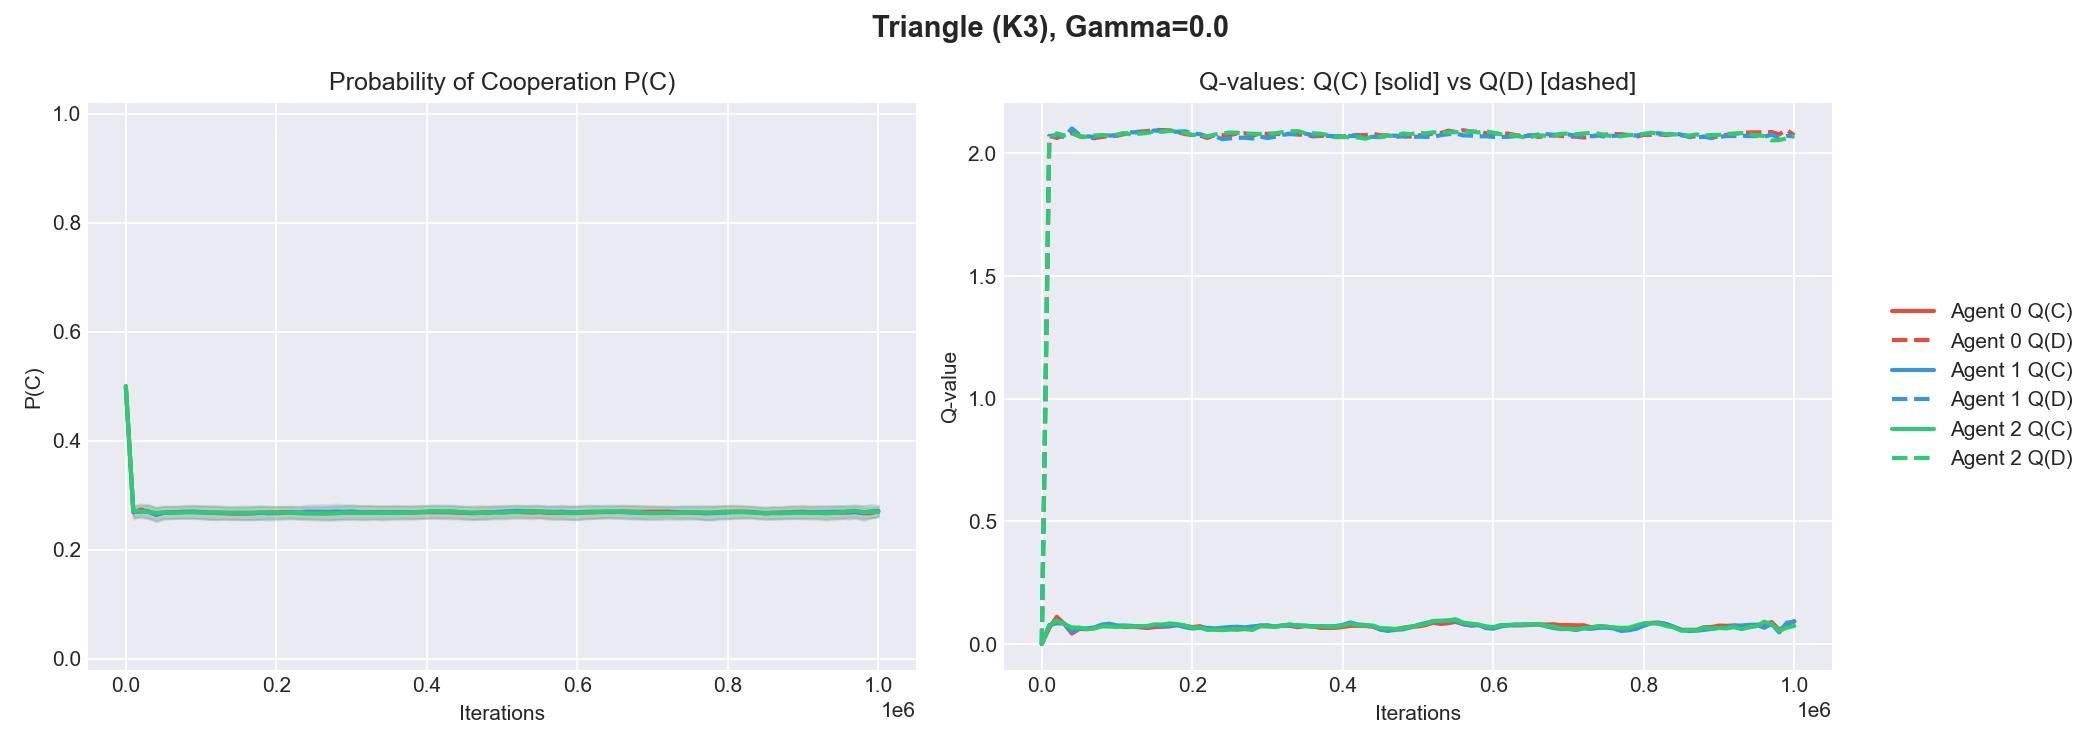
\includegraphics[width=\linewidth]{figures/triangle_gamma0.0.jpg}
	\caption{Динамика вероятности выбора действия C $p_i^{(t)}(C)$ и Q-значений $Q_i^{(t)}(a)$ алгоритма Q-обучения при $\gamma=0.0$. $T=1000000$, $\alpha = 0.01, \beta = 0.5$.}
\end{figure}

\begin{figure} [H]
	\centering
	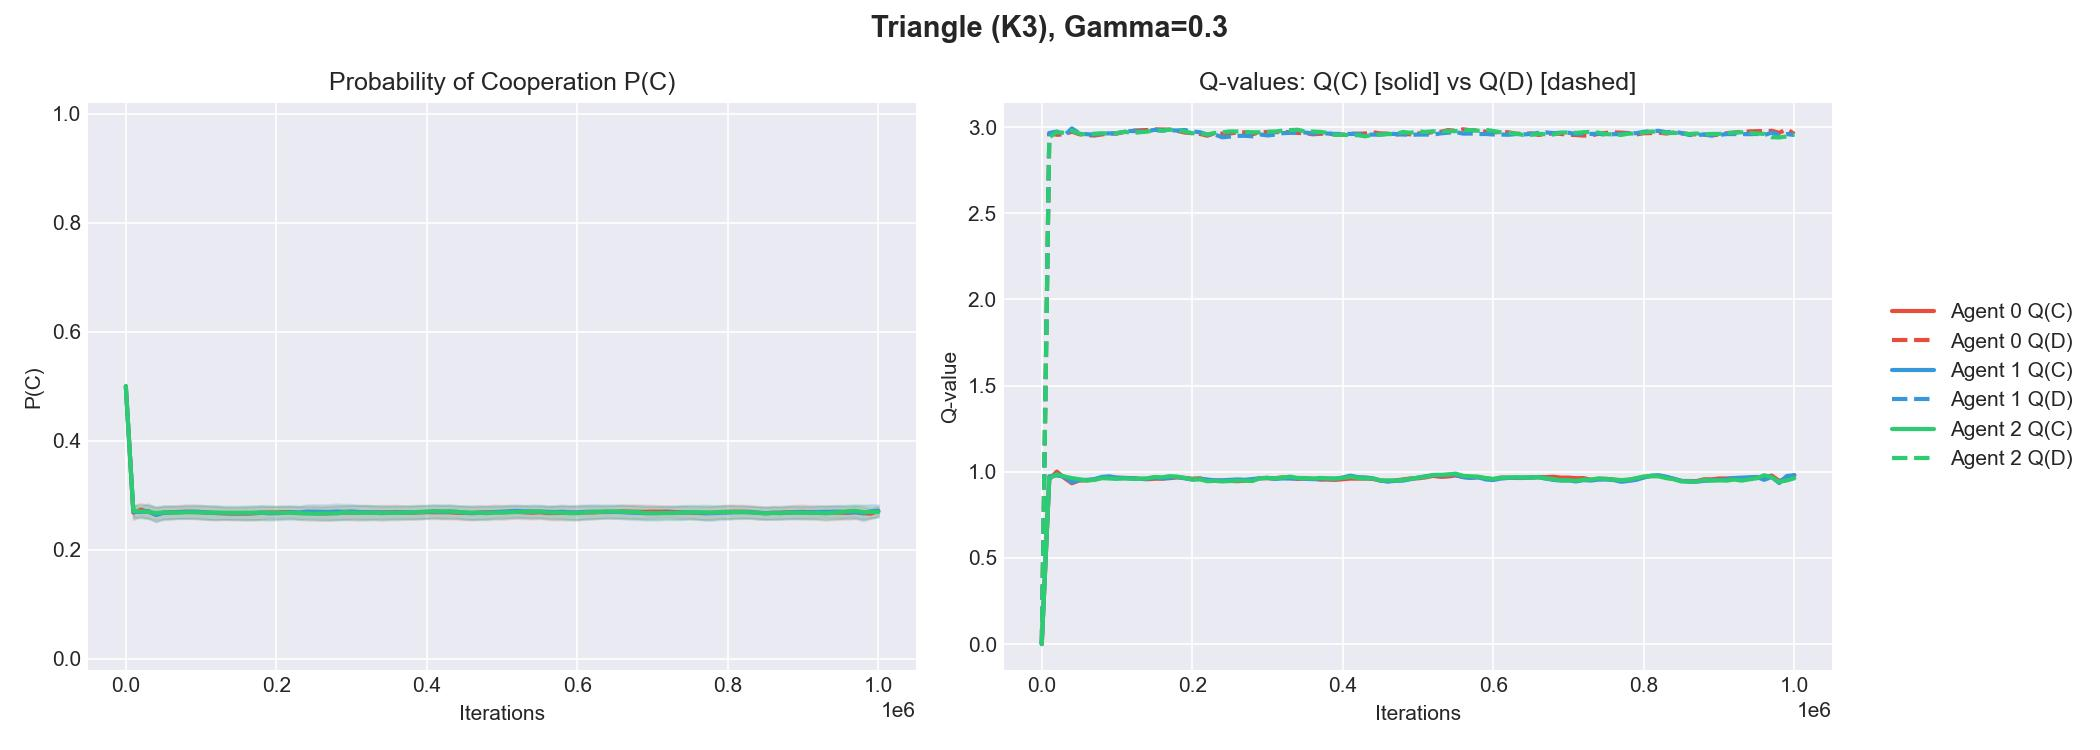
\includegraphics[width=\linewidth]{figures/triangle_gamma0.3.jpg}
	\caption{Динамика вероятности выбора действия C $p_i^{(t)}(C)$ и Q-значений $Q_i^{(t)}(a)$ алгоритма Q-обучения при $\gamma=0.3$. $T=1000000$, $\alpha = 0.01, \beta = 0.5$.}
\end{figure}

\begin{figure} [H]
	\centering
	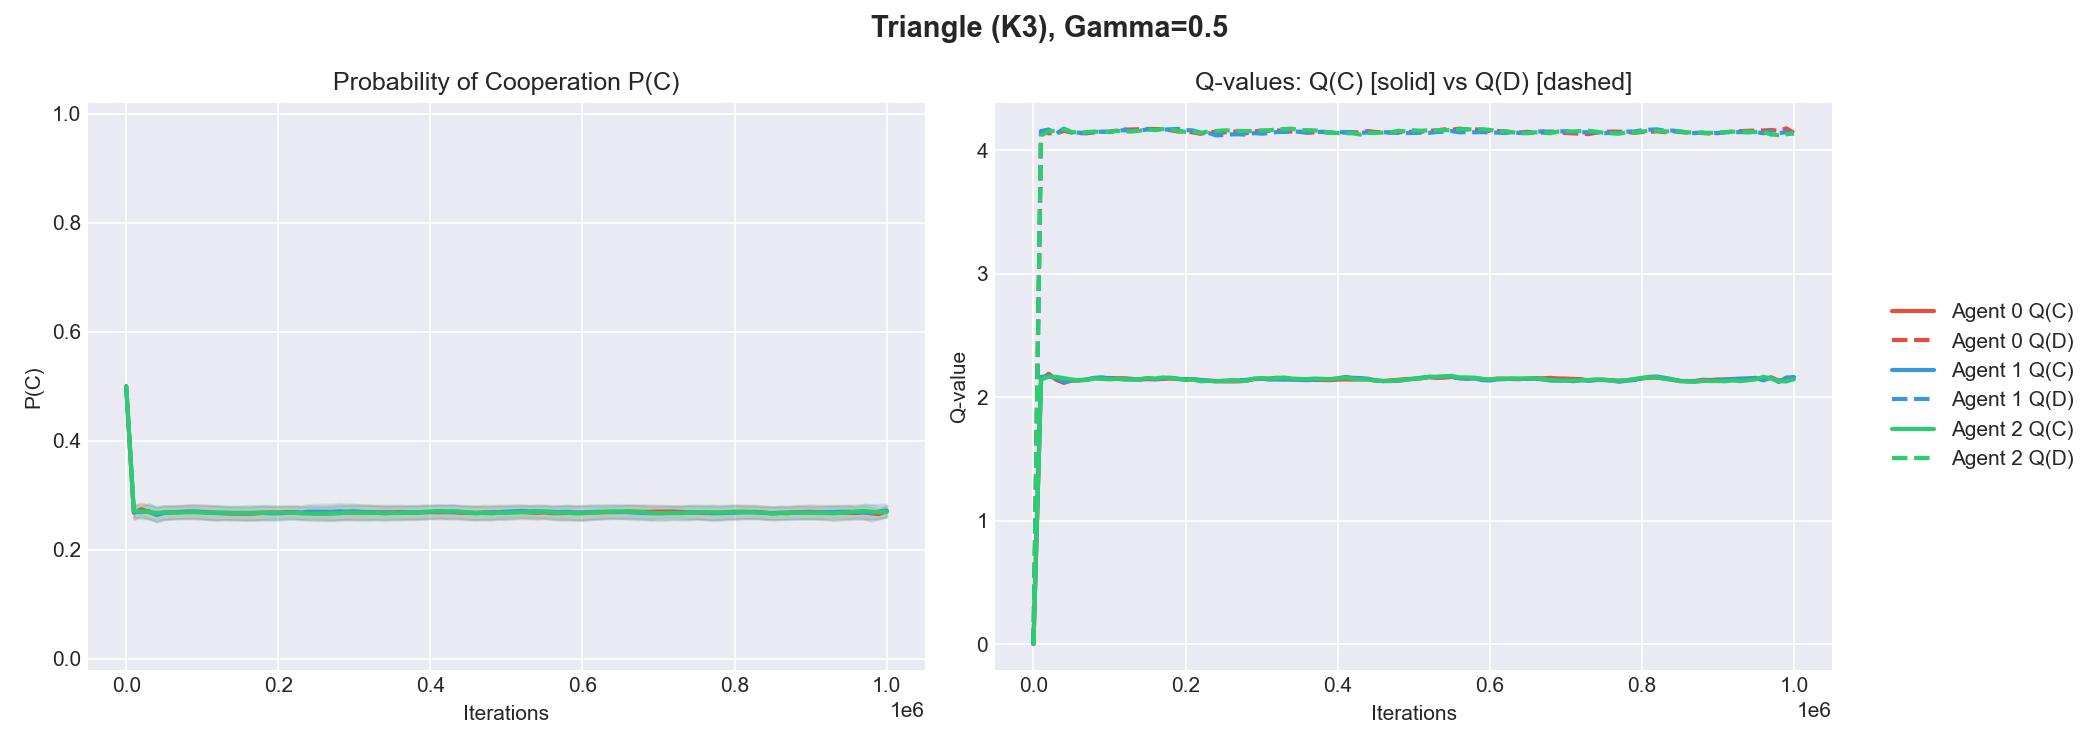
\includegraphics[width=\linewidth]{figures/triangle_gamma0.5.jpg}
	\caption{Динамика вероятности выбора действия C $p_i^{(t)}(C)$ и Q-значений $Q_i^{(t)}(a)$ алгоритма Q-обучения при $\gamma=0.5$. $T=1000000$, $\alpha = 0.01, \beta = 0.5$.}
\end{figure}

\begin{figure} [H]
	\centering
	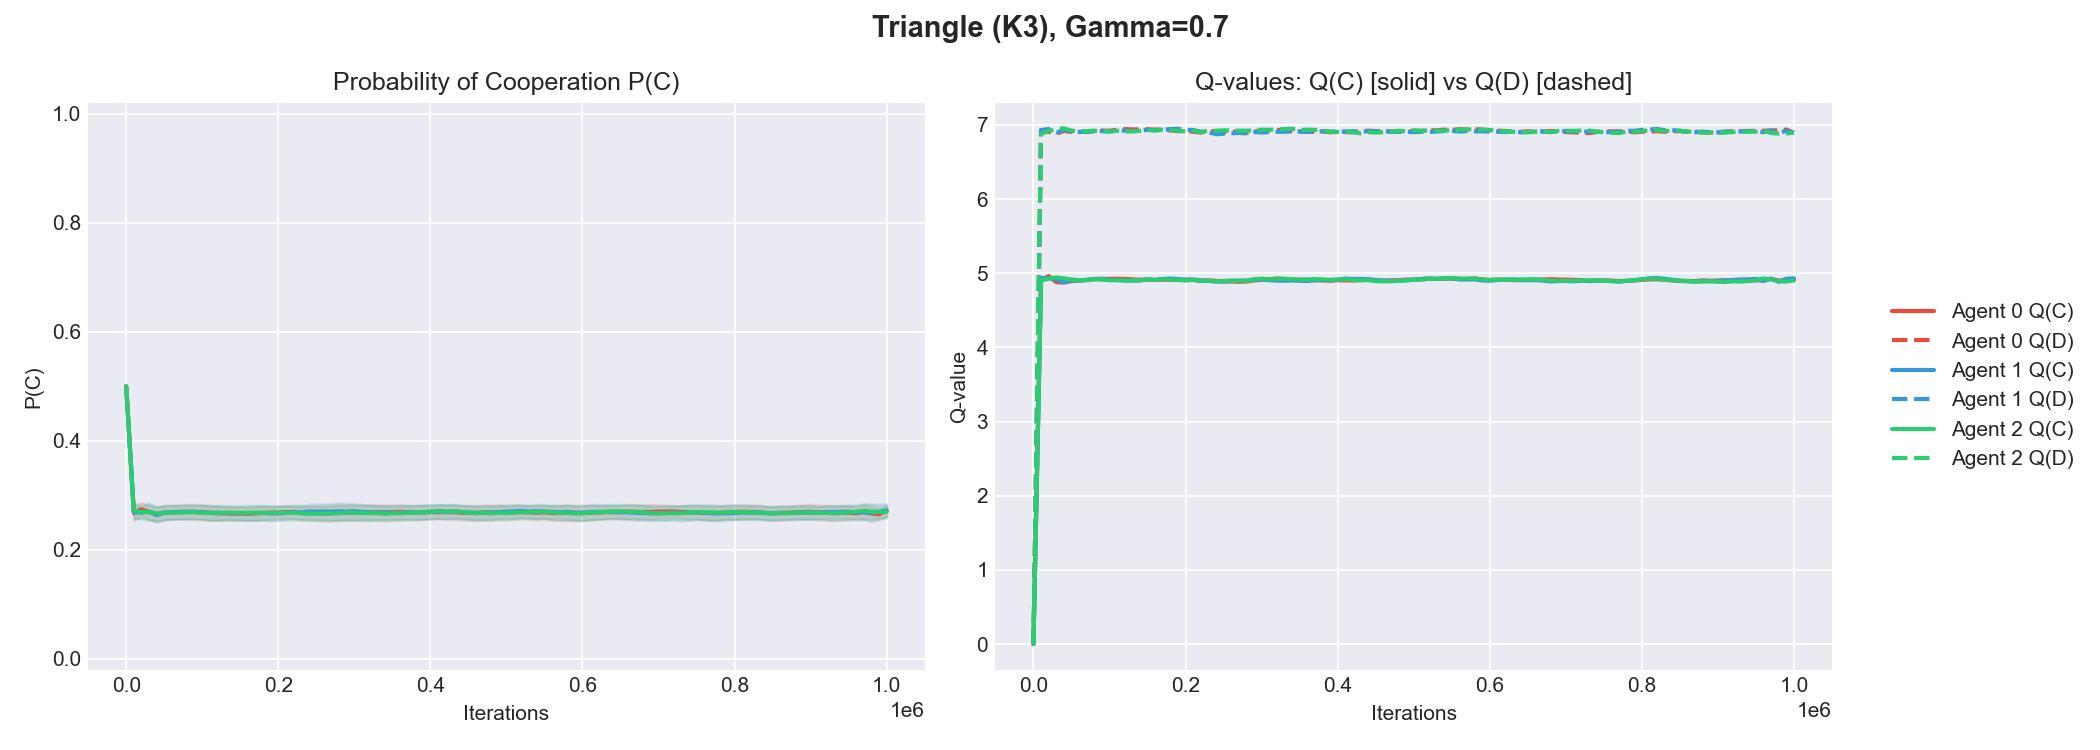
\includegraphics[width=\linewidth]{figures/triangle_gamma0.7.jpg}
	\caption{Динамика вероятности выбора действия C $p_i^{(t)}(C)$ и Q-значений $Q_i^{(t)}(a)$ алгоритма Q-обучения при $\gamma=0.7$. $T=1000000$, $\alpha = 0.01, \beta = 0.5$.}
\end{figure}

\begin{figure} [H]
	\centering
	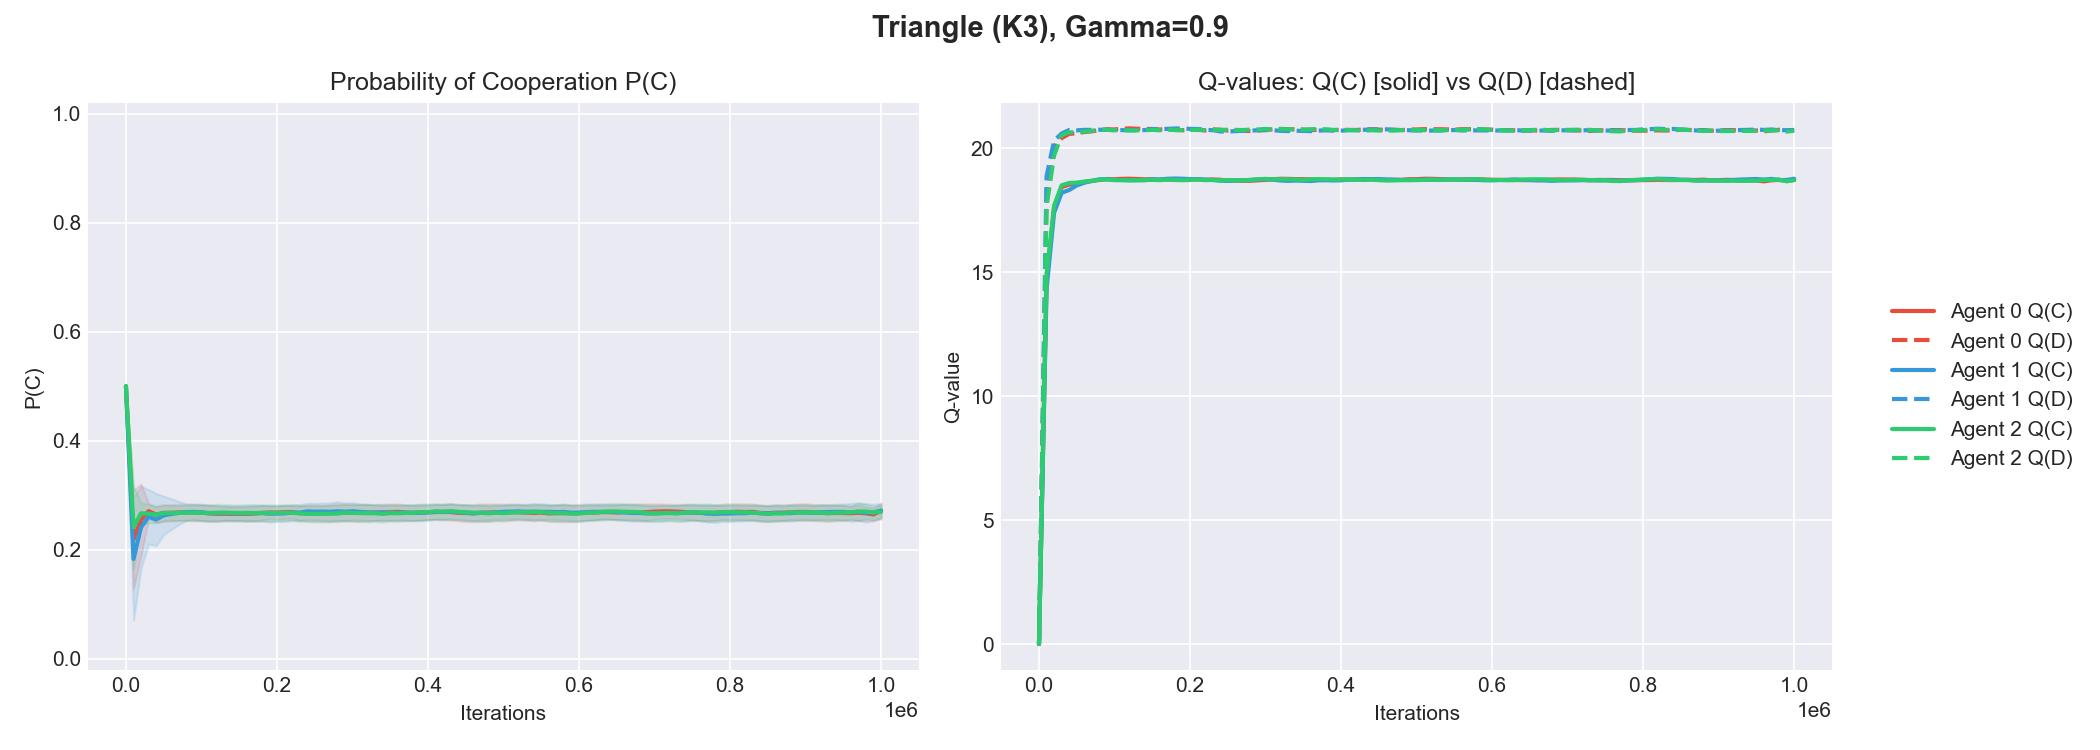
\includegraphics[width=\linewidth]{figures/triangle_gamma0.9.jpg}
	\caption{Динамика вероятности выбора действия C $p_i^{(t)}(C)$ и Q-значений $Q_i^{(t)}(a)$ алгоритма Q-обучения при $\gamma=0.9$. $T=1000000$, $\alpha = 0.01, \beta = 0.5$.}
\end{figure}

\subsubsection{Линия}

\begin{figure} [H]
	\centering
	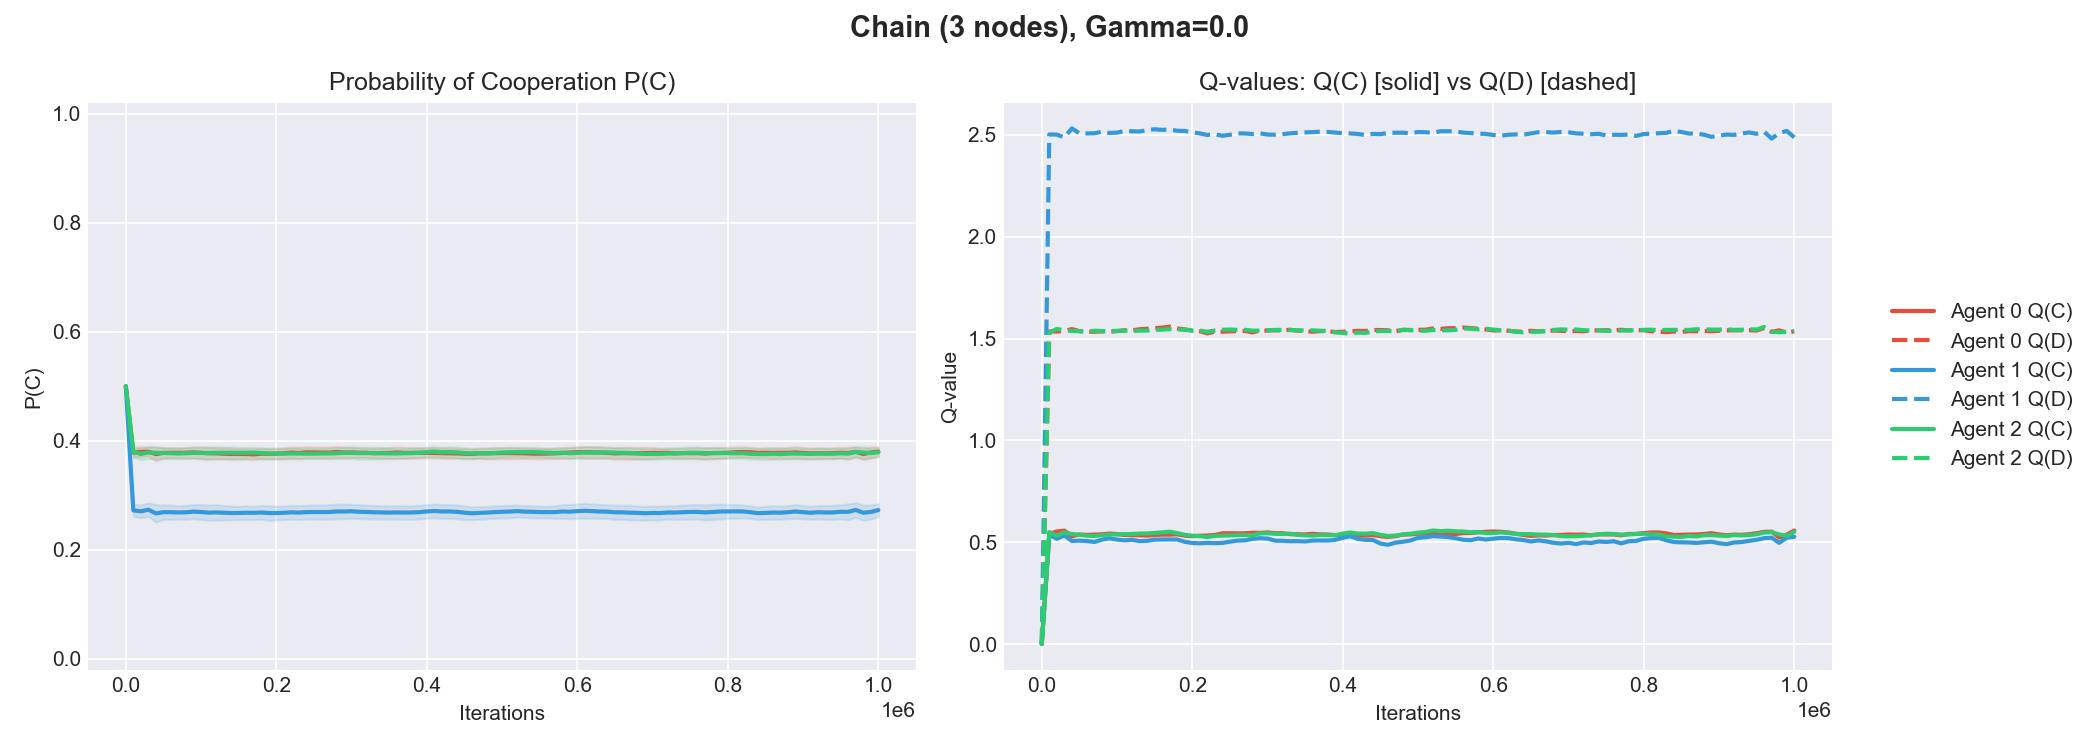
\includegraphics[width=\linewidth]{figures/chain3_gamma0.0.jpg}
	\caption{Динамика вероятности выбора действия C $p_i^{(t)}(C)$ и Q-значений $Q_i^{(t)}(a)$ алгоритма Q-обучения при $\gamma=0.0$. $T=1000000$, $\alpha = 0.01, \beta = 0.5$.}
\end{figure}

\begin{figure} [H]
	\centering
	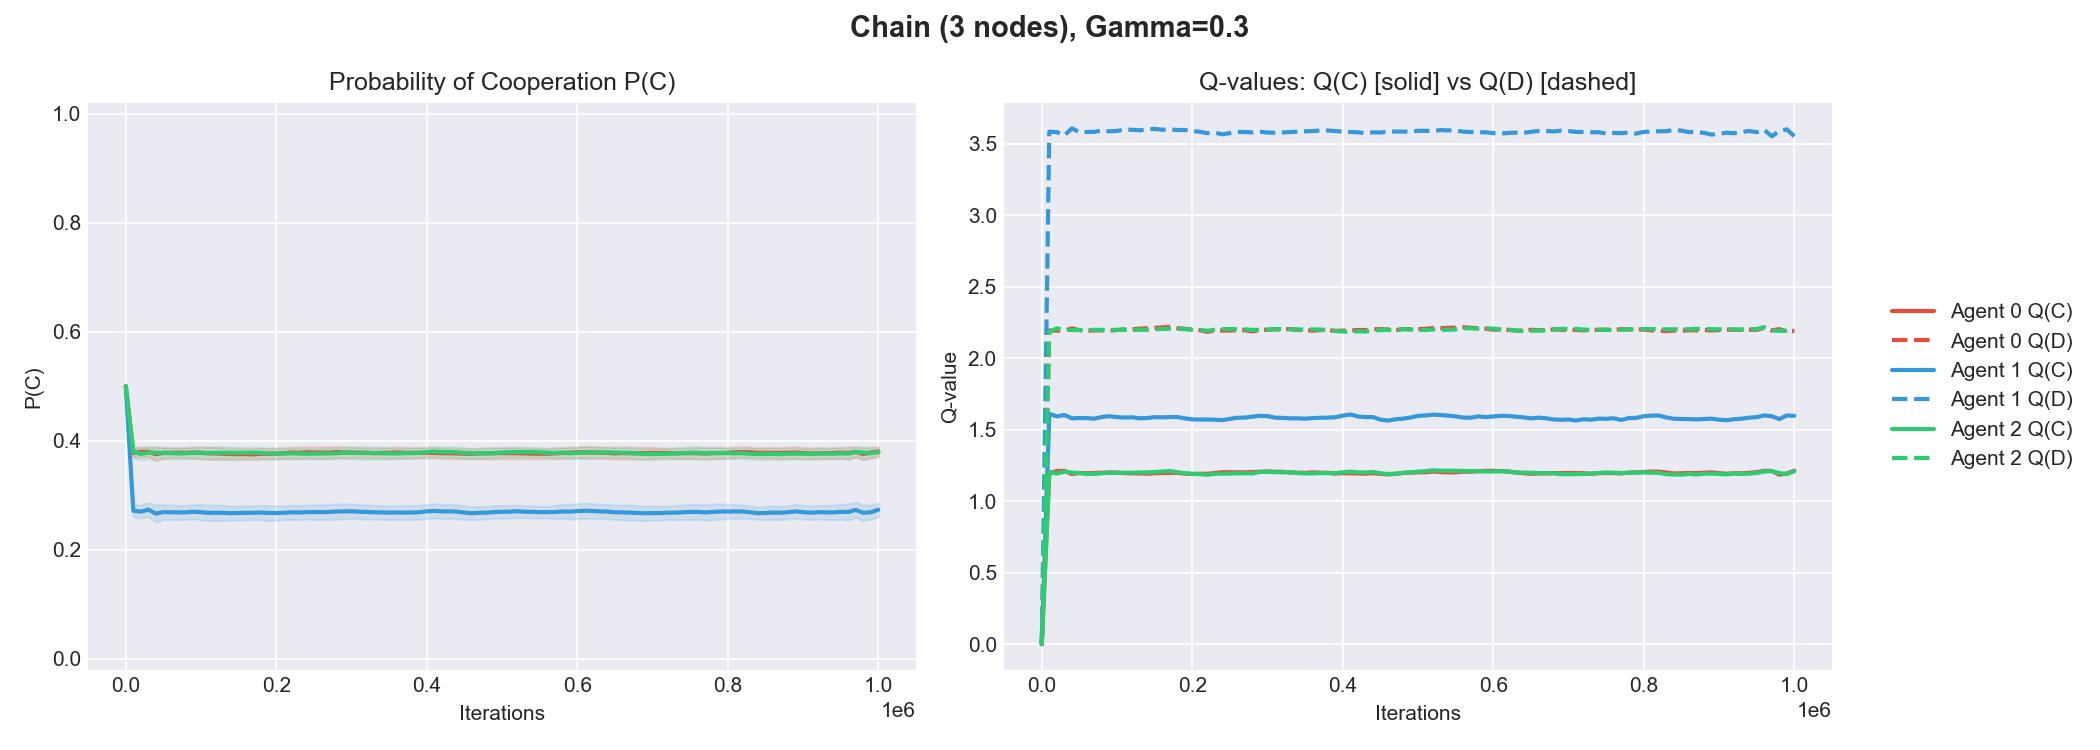
\includegraphics[width=\linewidth]{figures/chain3_gamma0.3.jpg}
	\caption{Динамика вероятности выбора действия C $p_i^{(t)}(C)$ и Q-значений $Q_i^{(t)}(a)$ алгоритма Q-обучения при $\gamma=0.3$. $T=1000000$, $\alpha = 0.01, \beta = 0.5$.}
\end{figure}

\begin{figure} [H]
	\centering
	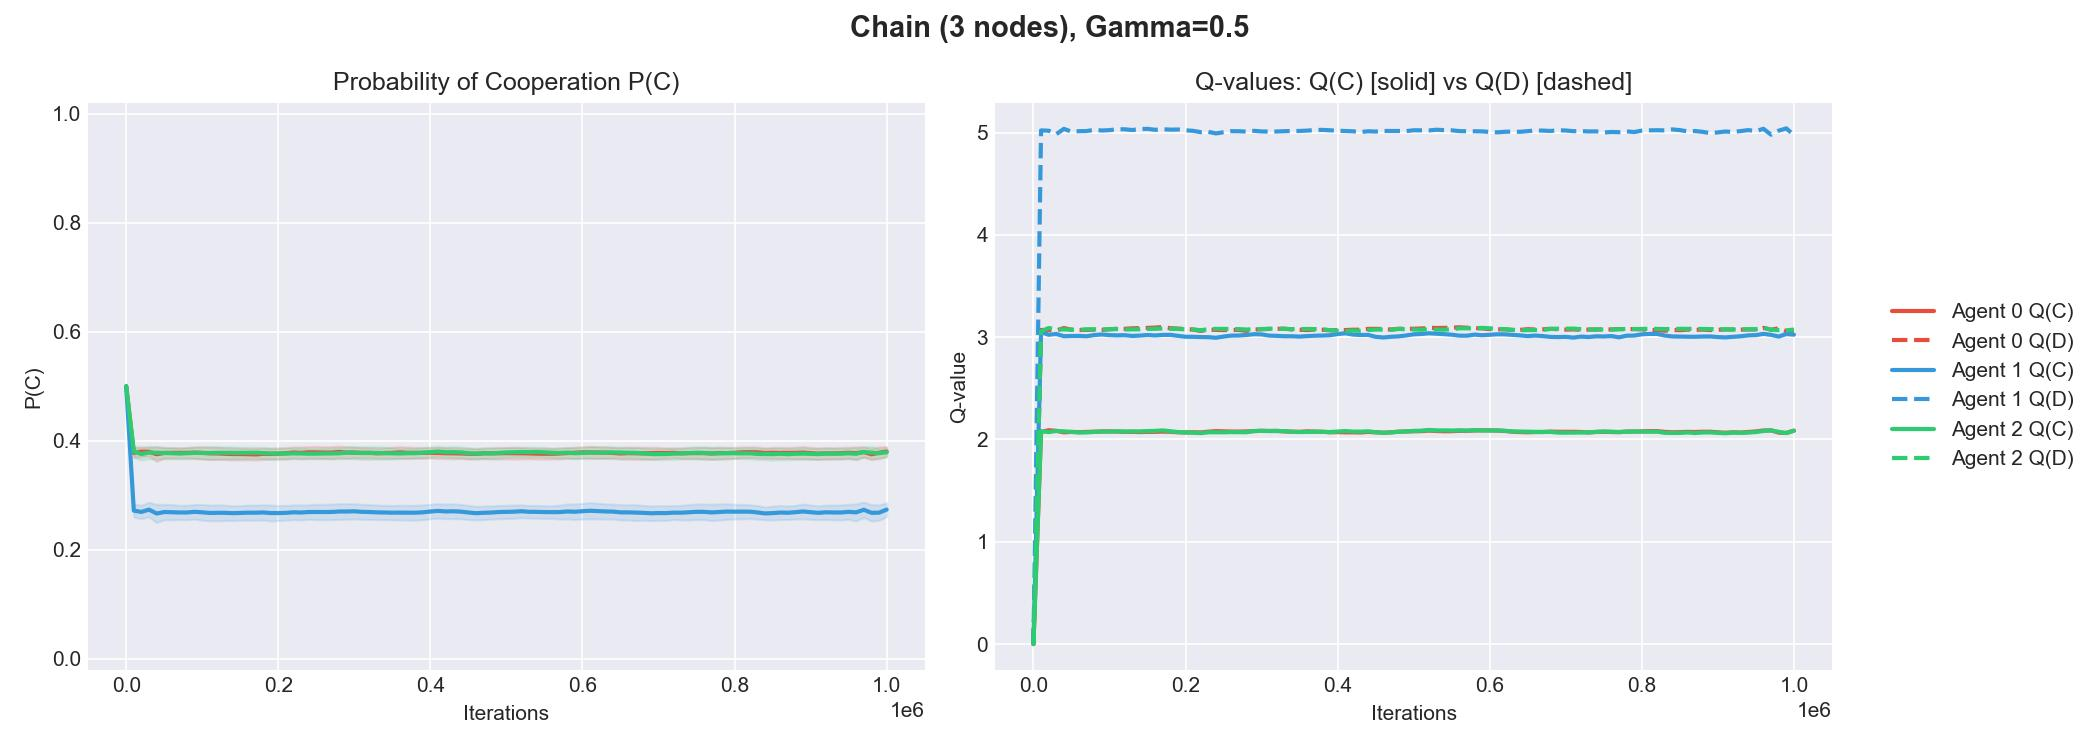
\includegraphics[width=\linewidth]{figures/chain3_gamma0.5.jpg}
	\caption{Динамика вероятности выбора действия C $p_i^{(t)}(C)$ и Q-значений $Q_i^{(t)}(a)$ алгоритма Q-обучения при $\gamma=0.5$. $T=1000000$, $\alpha = 0.01, \beta = 0.5$.}
\end{figure}

\begin{figure} [H]
	\centering
	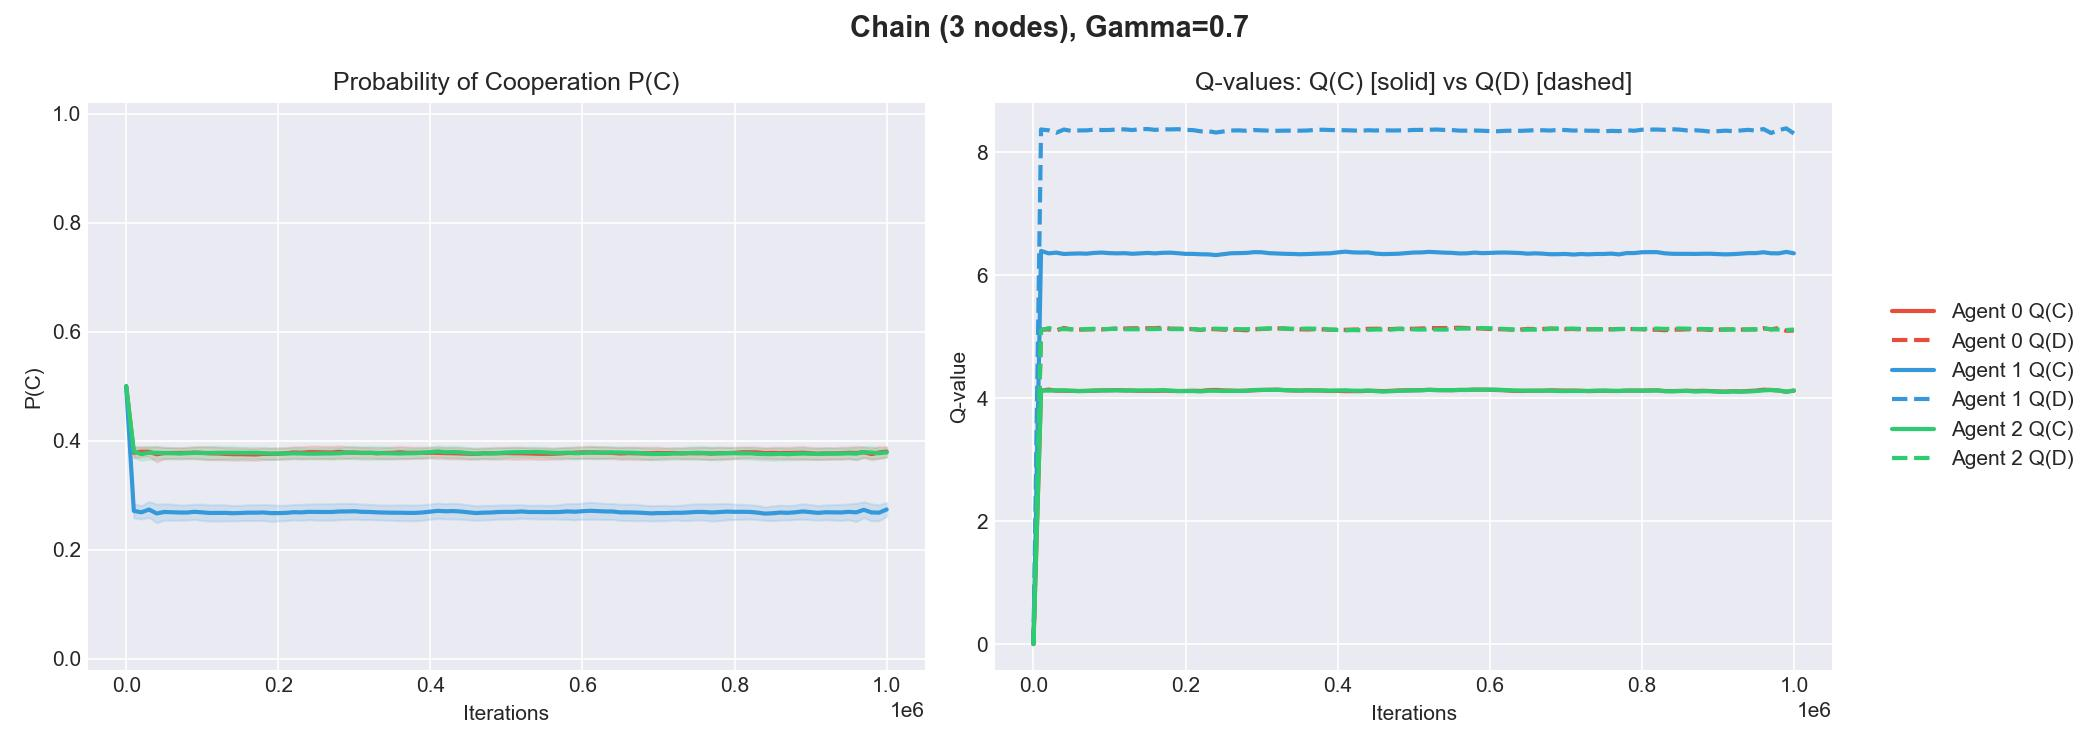
\includegraphics[width=\linewidth]{figures/chain3_gamma0.7.jpg}
	\caption{Динамика вероятности выбора действия C $p_i^{(t)}(C)$ и Q-значений $Q_i^{(t)}(a)$ алгоритма Q-обучения при $\gamma=0.7$. $T=1000000$, $\alpha = 0.01, \beta = 0.5$.}
\end{figure}

\begin{figure} [H]
	\centering
	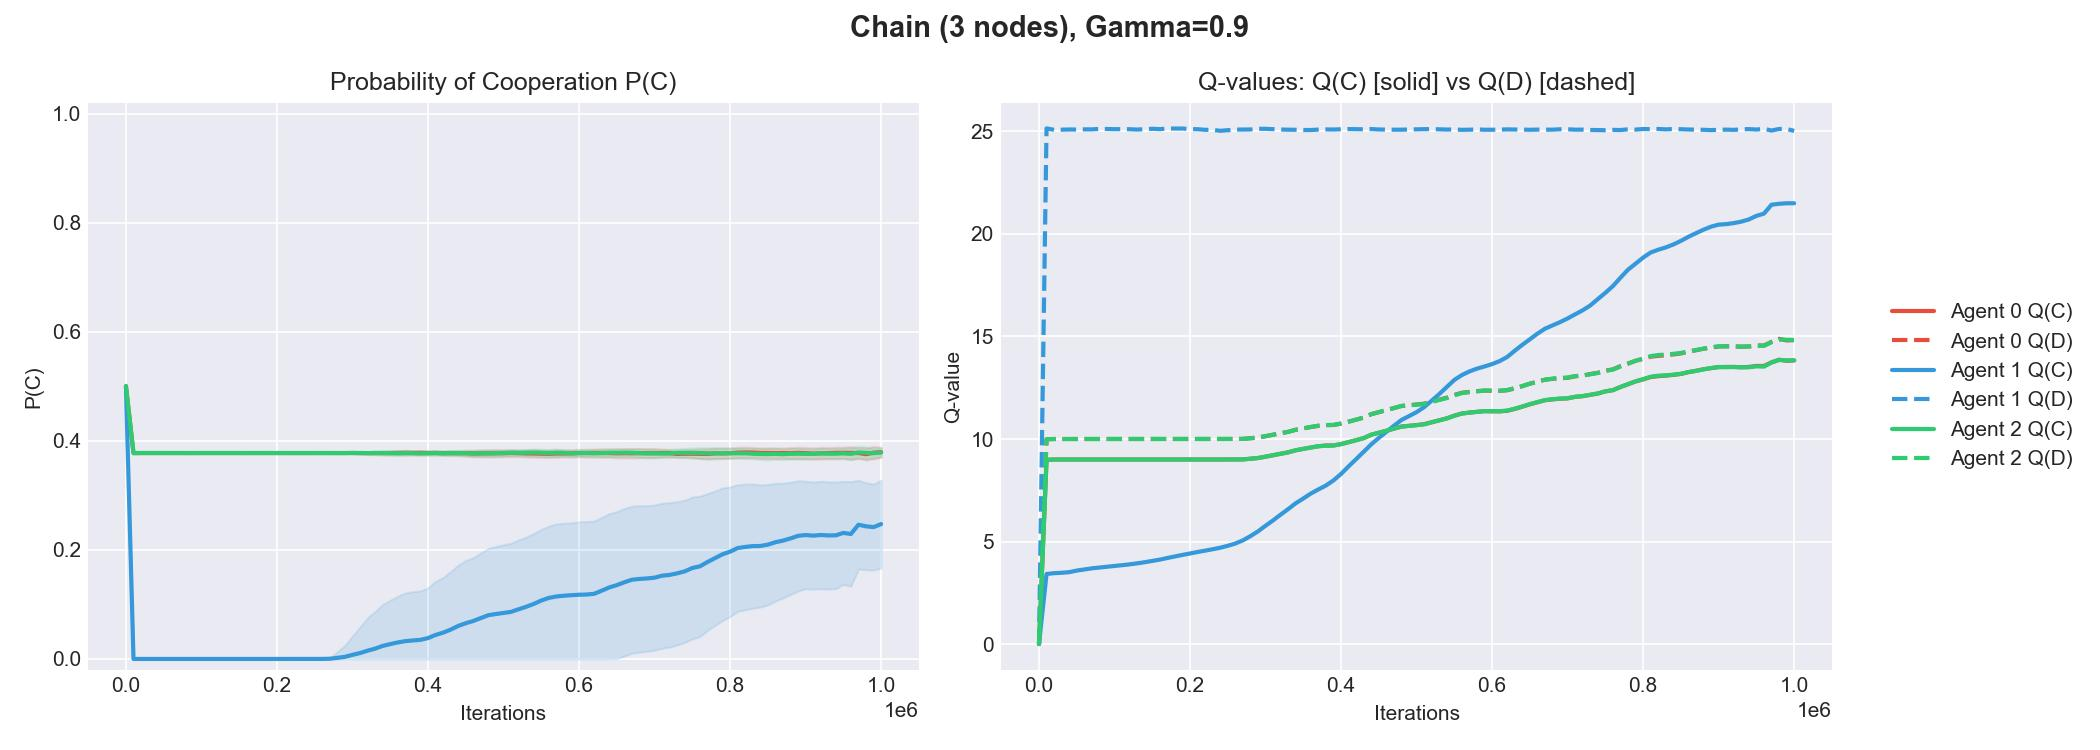
\includegraphics[width=\linewidth]{figures/chain3_gamma0.9.jpg}
	\caption{Динамика вероятности выбора действия C $p_i^{(t)}(C)$ и Q-значений $Q_i^{(t)}(a)$ алгоритма Q-обучения при $\gamma=0.9$. $T=1000000$, $\alpha = 0.01, \beta = 0.5$.}
\end{figure}

\subsection{Граф с 4 вершинами}

\subsubsection{Клика}

\begin{figure} [H]
	\centering
	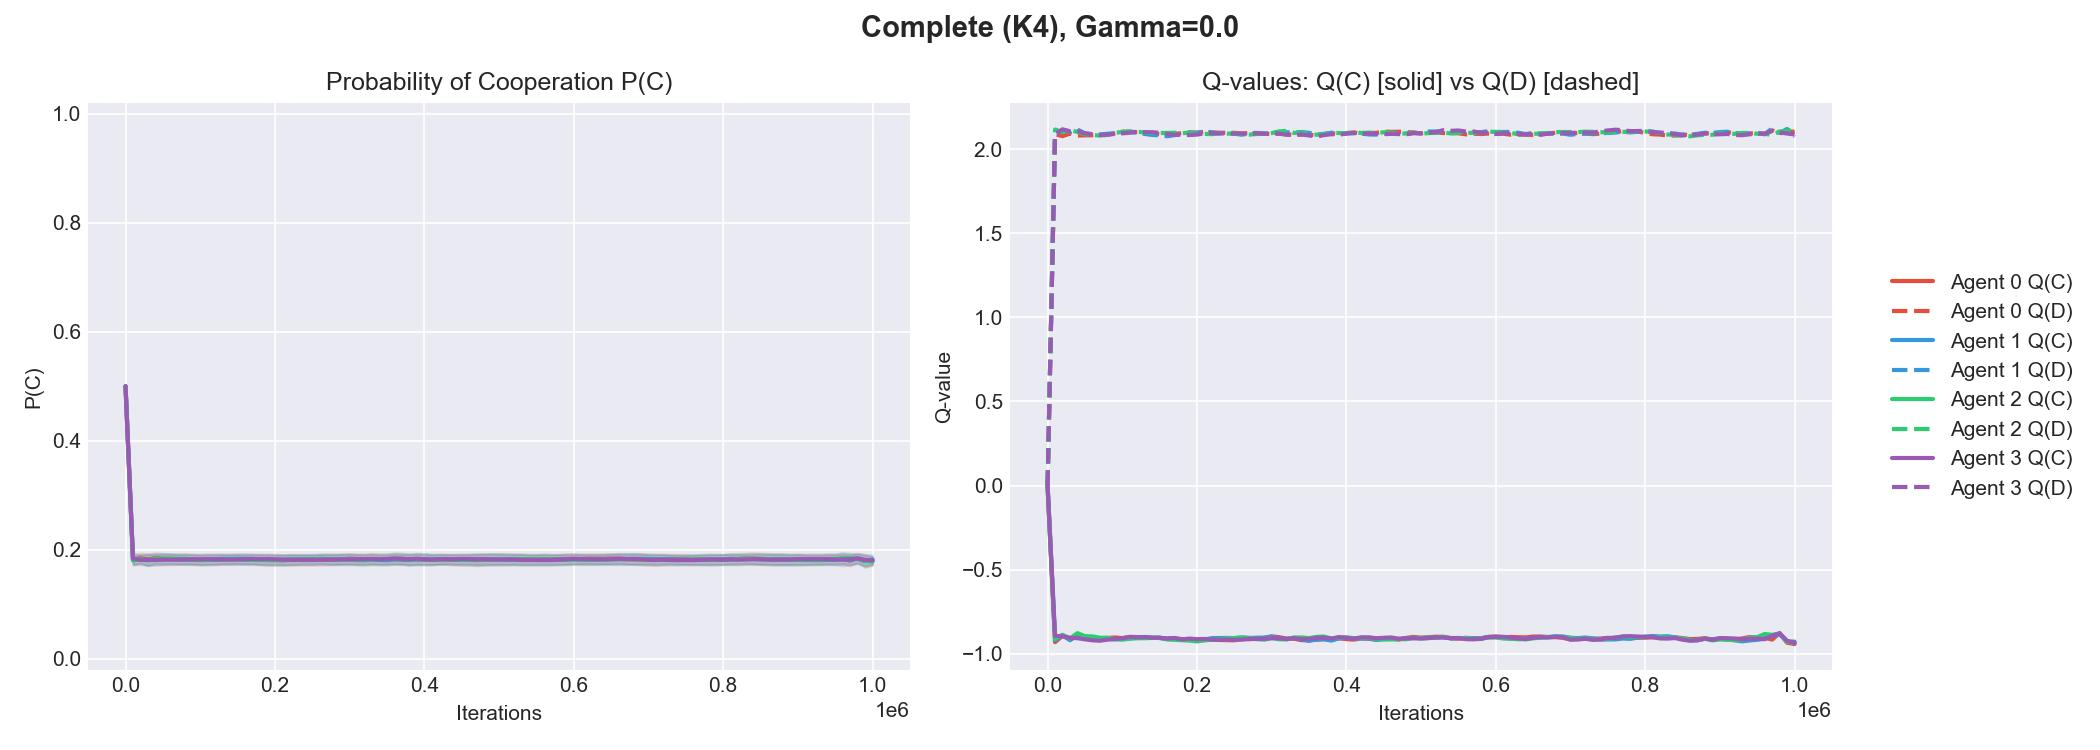
\includegraphics[width=\linewidth]{figures/complete4_gamma0.0.jpg}
	\caption{Динамика вероятности выбора действия C $p_i^{(t)}(C)$ и Q-значений $Q_i^{(t)}(a)$ алгоритма Q-обучения при $\gamma=0.0$. $T=1000000$, $\alpha = 0.01, \beta = 0.5$.}
\end{figure}

\begin{figure} [H]
	\centering
	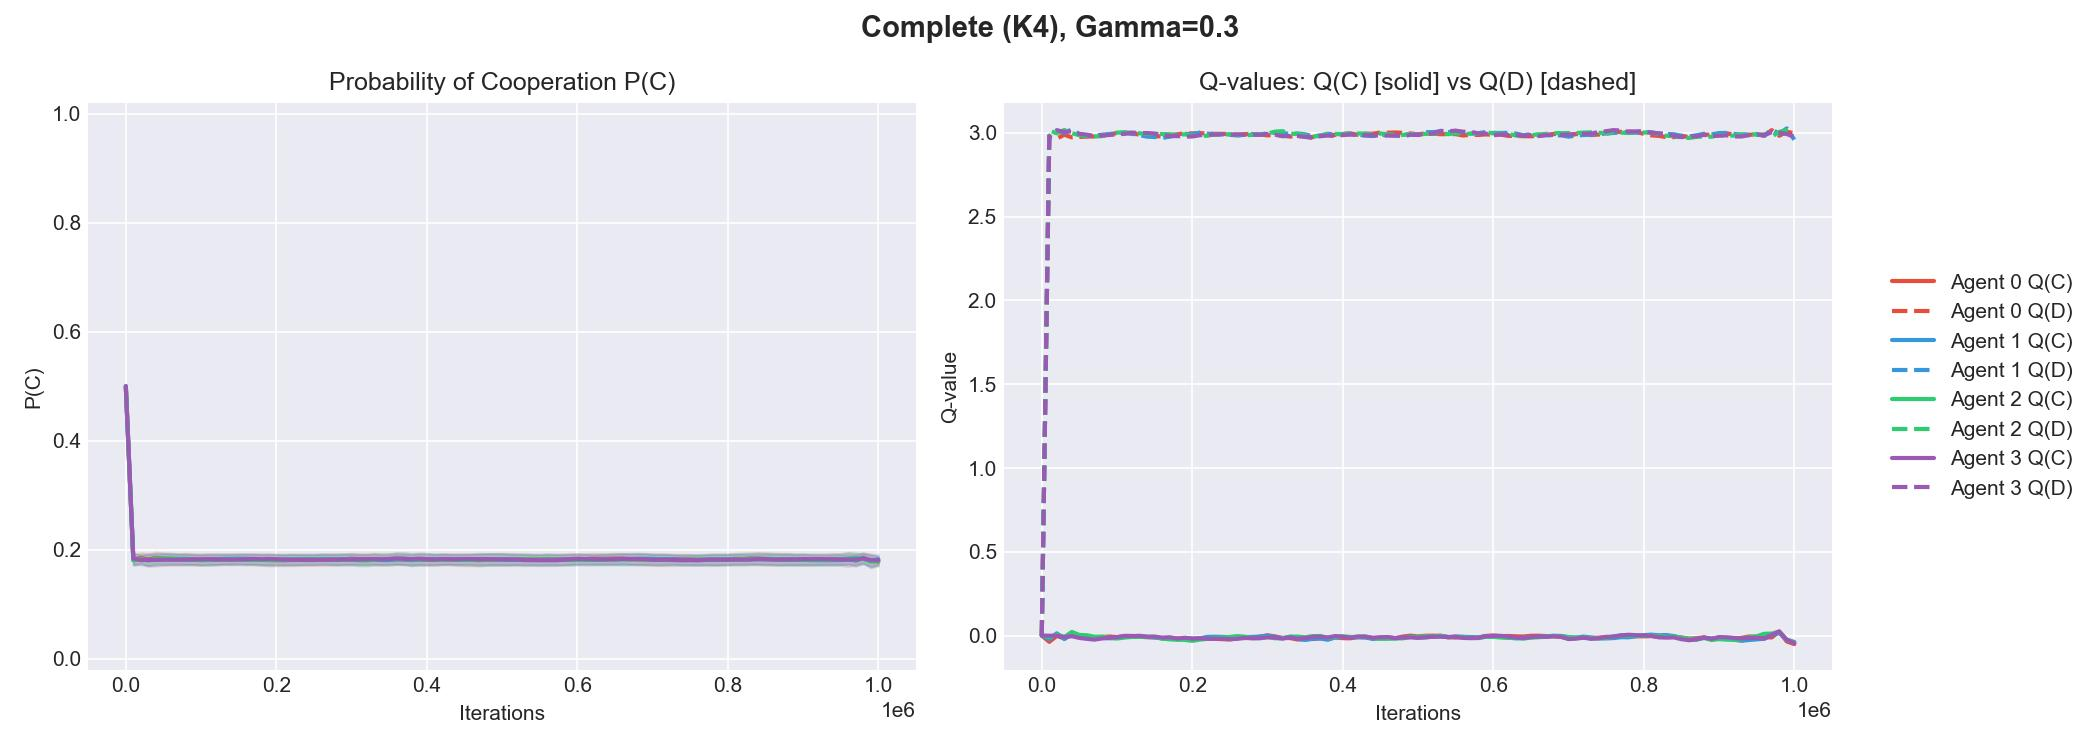
\includegraphics[width=\linewidth]{figures/complete4_gamma0.3.jpg}
	\caption{Динамика вероятности выбора действия C $p_i^{(t)}(C)$ и Q-значений $Q_i^{(t)}(a)$ алгоритма Q-обучения при $\gamma=0.3$. $T=1000000$, $\alpha = 0.01, \beta = 0.5$.}
\end{figure}

\begin{figure} [H]
	\centering
	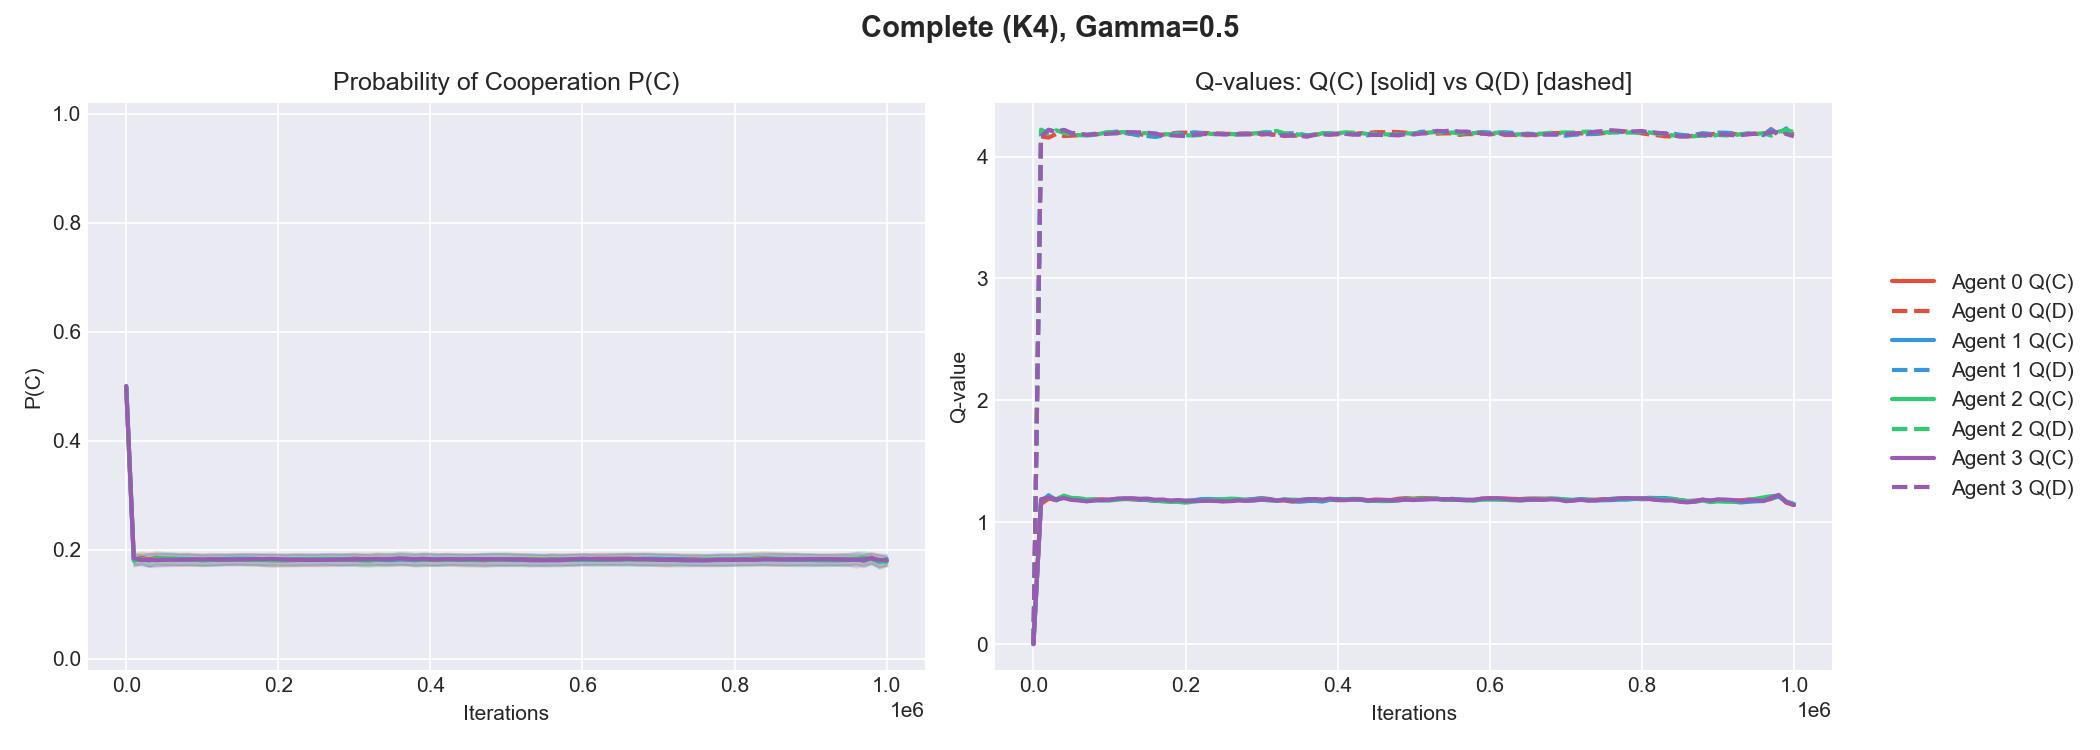
\includegraphics[width=\linewidth]{figures/complete4_gamma0.5.jpg}
	\caption{Динамика вероятности выбора действия C $p_i^{(t)}(C)$ и Q-значений $Q_i^{(t)}(a)$ алгоритма Q-обучения при $\gamma=0.5$. $T=1000000$, $\alpha = 0.01, \beta = 0.5$.}
\end{figure}

\begin{figure} [H]
	\centering
	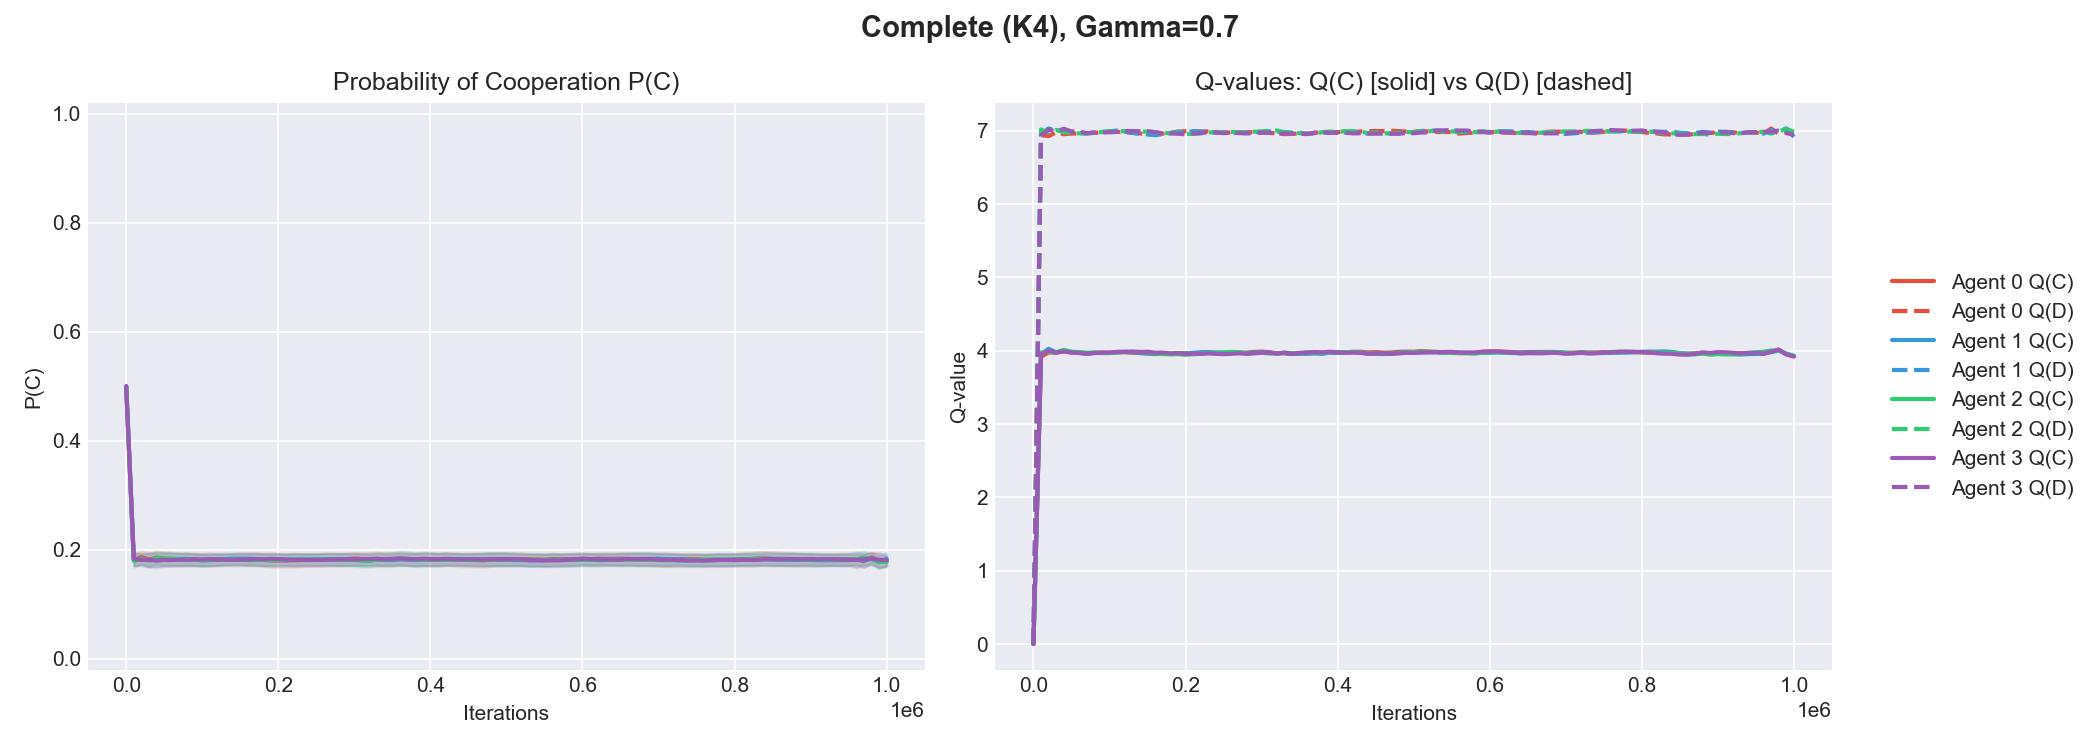
\includegraphics[width=\linewidth]{figures/complete4_gamma0.7.jpg}
	\caption{Динамика вероятности выбора действия C $p_i^{(t)}(C)$ и Q-значений $Q_i^{(t)}(a)$ алгоритма Q-обучения при $\gamma=0.7$. $T=1000000$, $\alpha = 0.01, \beta = 0.5$.}
\end{figure}

\begin{figure} [H]
	\centering
	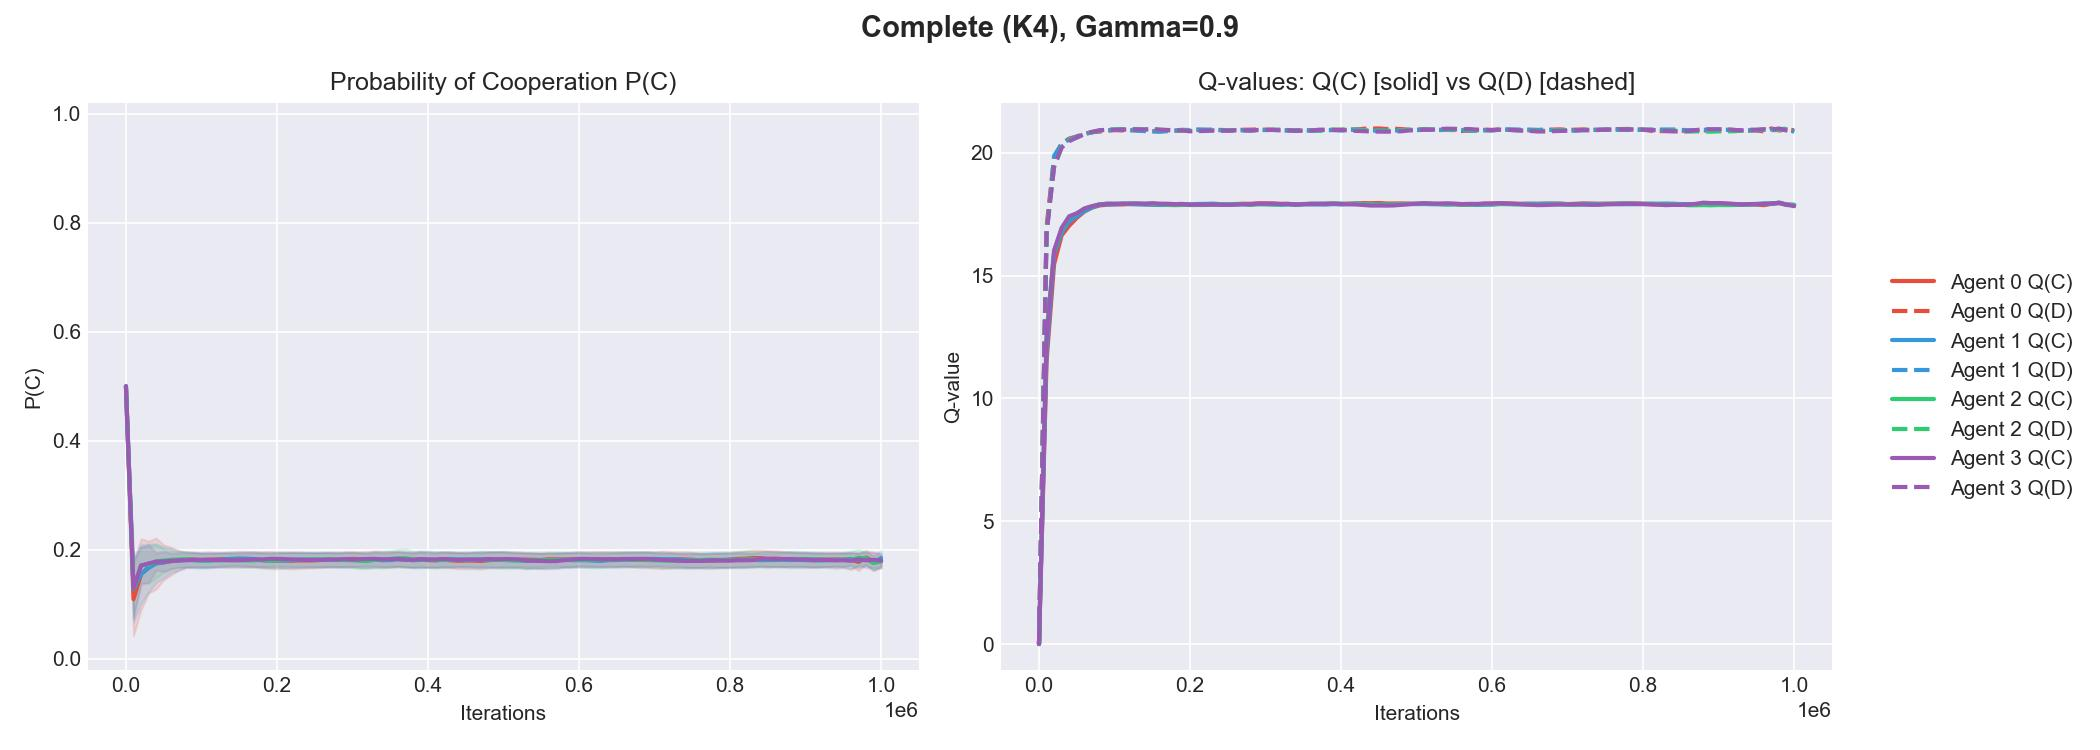
\includegraphics[width=\linewidth]{figures/complete4_gamma0.9.jpg}
	\caption{Динамика вероятности выбора действия C $p_i^{(t)}(C)$ и Q-значений $Q_i^{(t)}(a)$ алгоритма Q-обучения при $\gamma=0.9$. $T=1000000$, $\alpha = 0.01, \beta = 0.5$.}
\end{figure}

\subsubsection{Линия}

\begin{figure} [H]
	\centering
	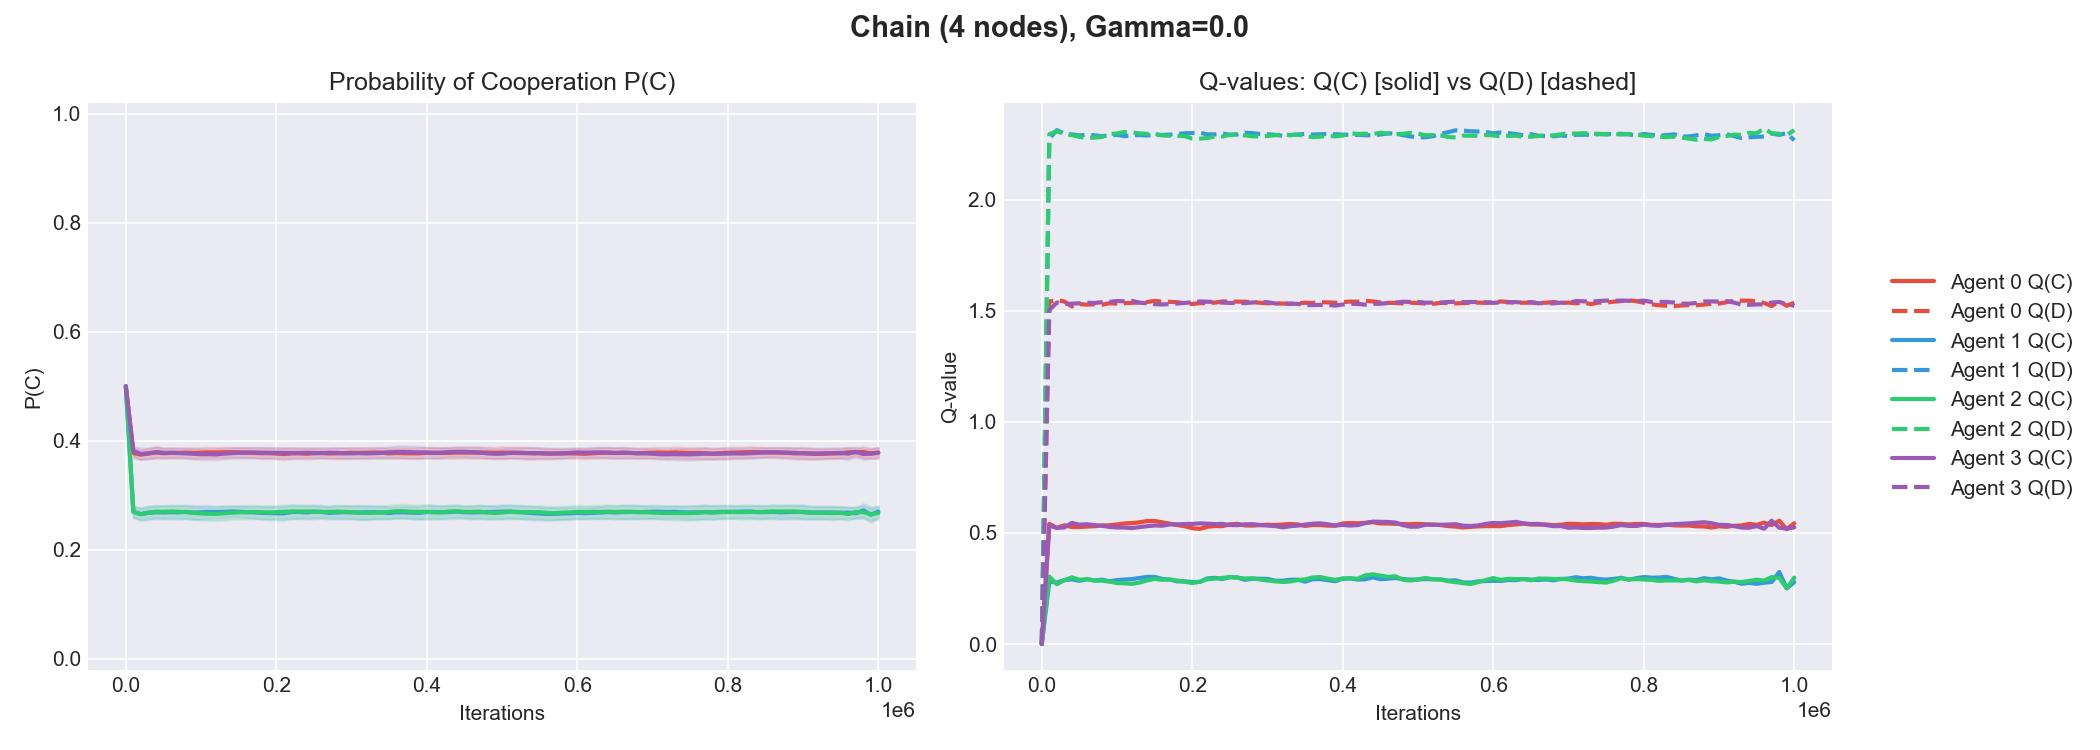
\includegraphics[width=\linewidth]{figures/chain4_gamma0.0.jpg}
	\caption{Динамика вероятности выбора действия C $p_i^{(t)}(C)$ и Q-значений $Q_i^{(t)}(a)$ алгоритма Q-обучения при $\gamma=0.0$. $T=1000000$, $\alpha = 0.01, \beta = 0.5$.}
\end{figure}

\begin{figure} [H]
	\centering
	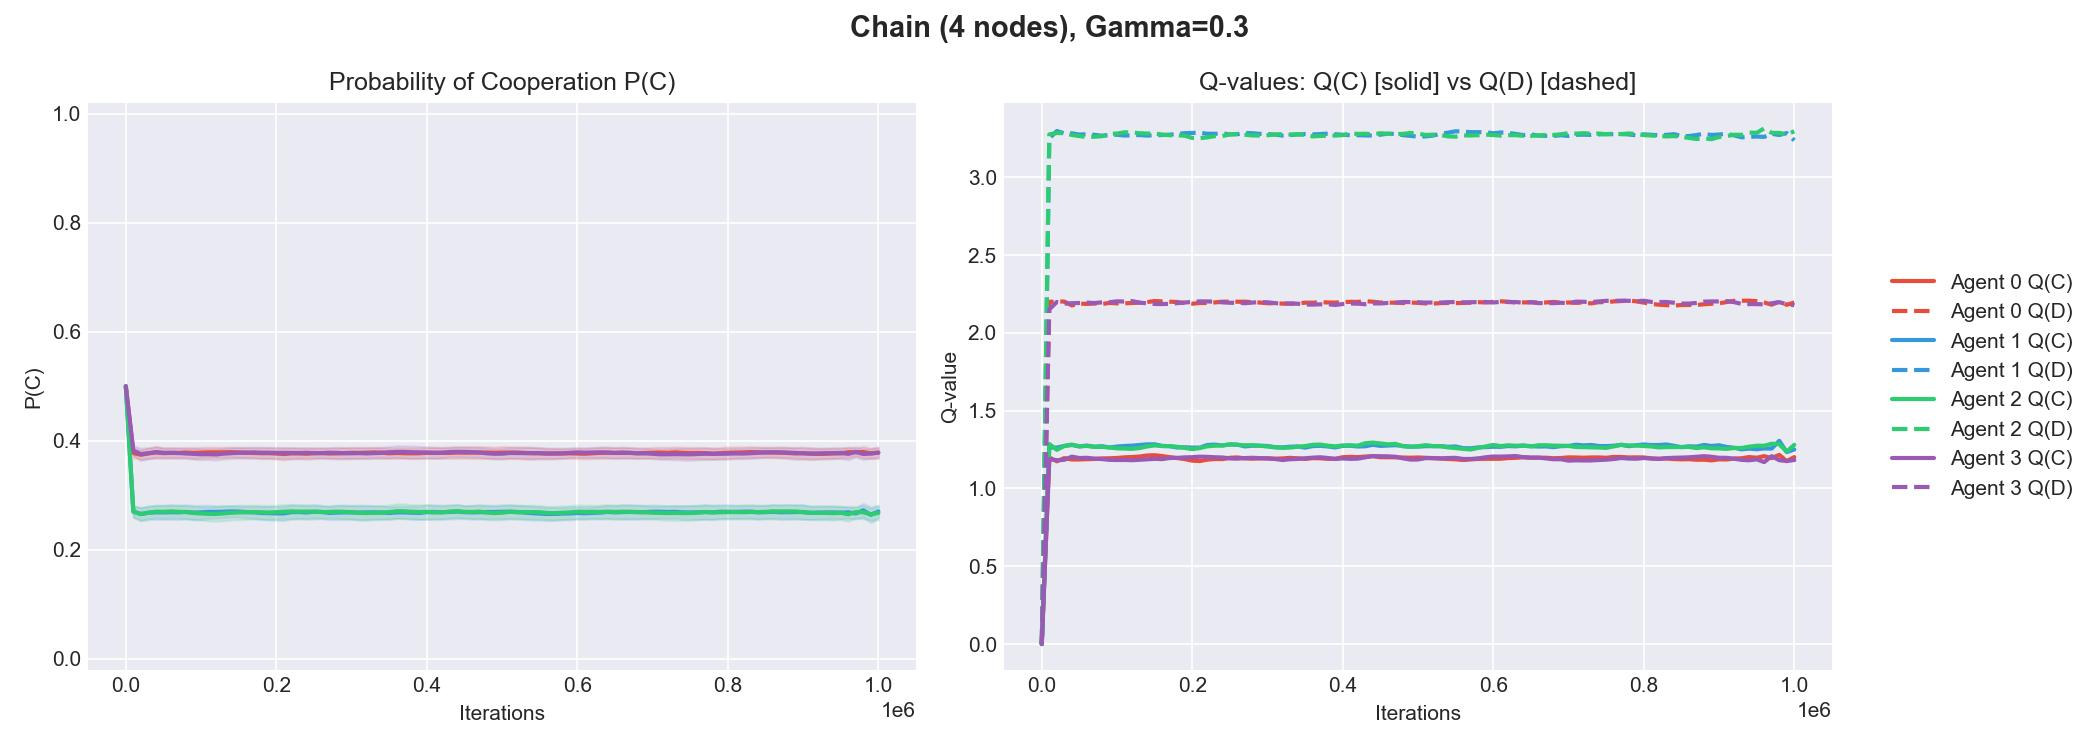
\includegraphics[width=\linewidth]{figures/chain4_gamma0.3.jpg}
	\caption{Динамика вероятности выбора действия C $p_i^{(t)}(C)$ и Q-значений $Q_i^{(t)}(a)$ алгоритма Q-обучения при $\gamma=0.3$. $T=1000000$, $\alpha = 0.01, \beta = 0.5$.}
\end{figure}

\begin{figure} [H]
	\centering
	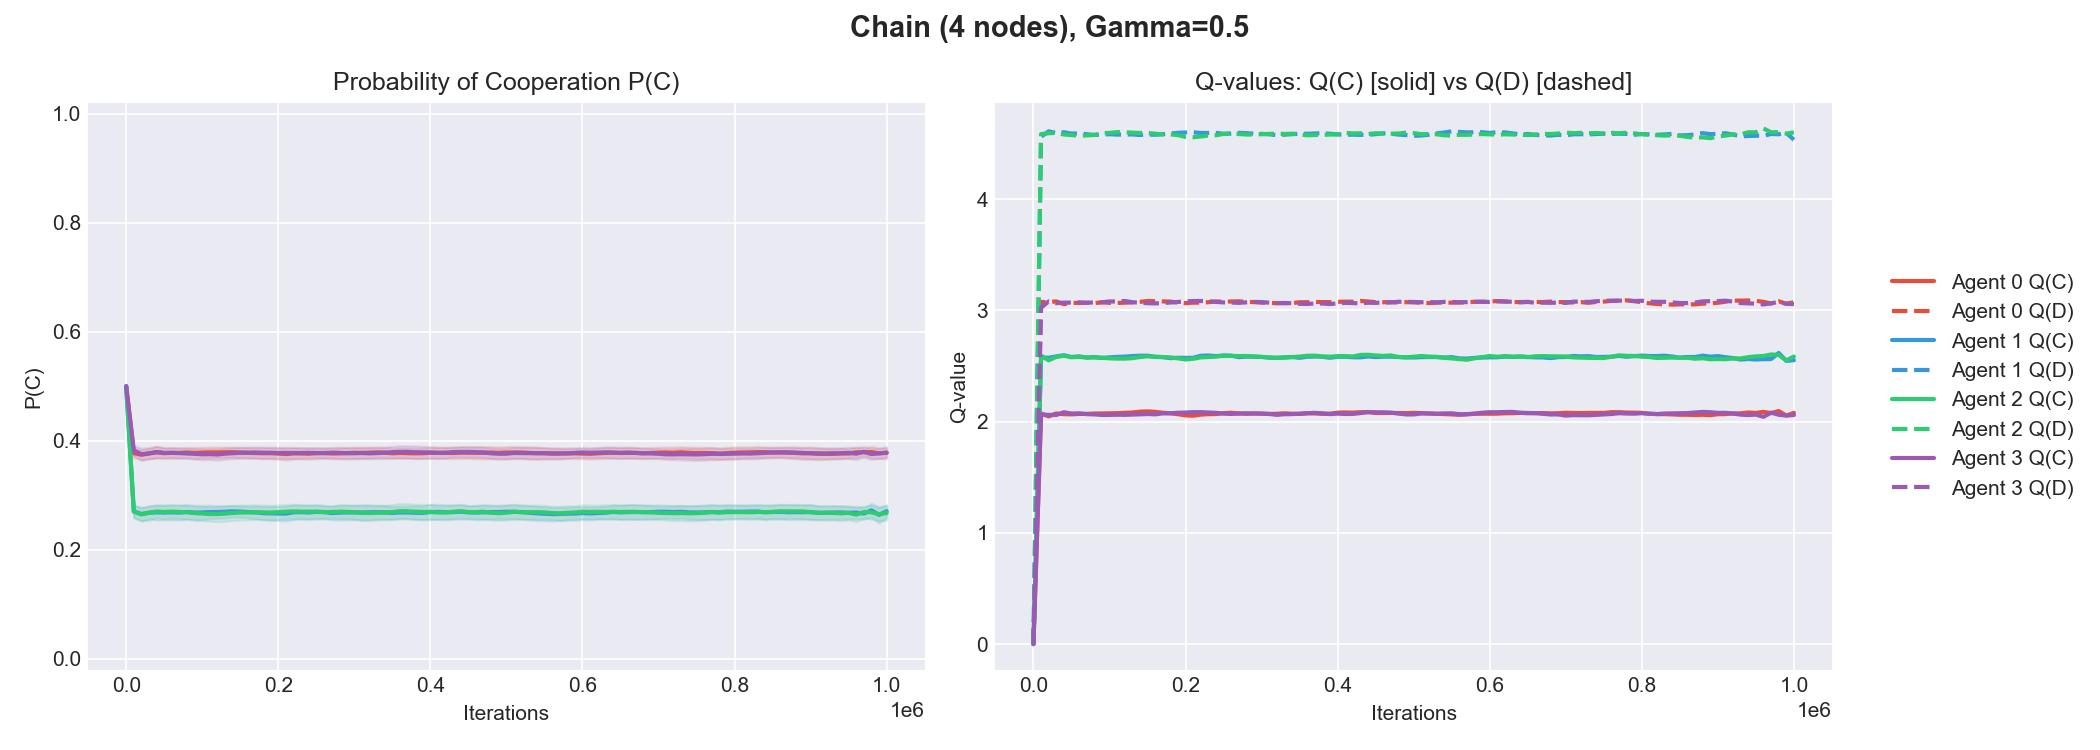
\includegraphics[width=\linewidth]{figures/chain4_gamma0.5.jpg}
	\caption{Динамика вероятности выбора действия C $p_i^{(t)}(C)$ и Q-значений $Q_i^{(t)}(a)$ алгоритма Q-обучения при $\gamma=0.5$. $T=1000000$, $\alpha = 0.01, \beta = 0.5$.}
\end{figure}

\begin{figure} [H]
	\centering
	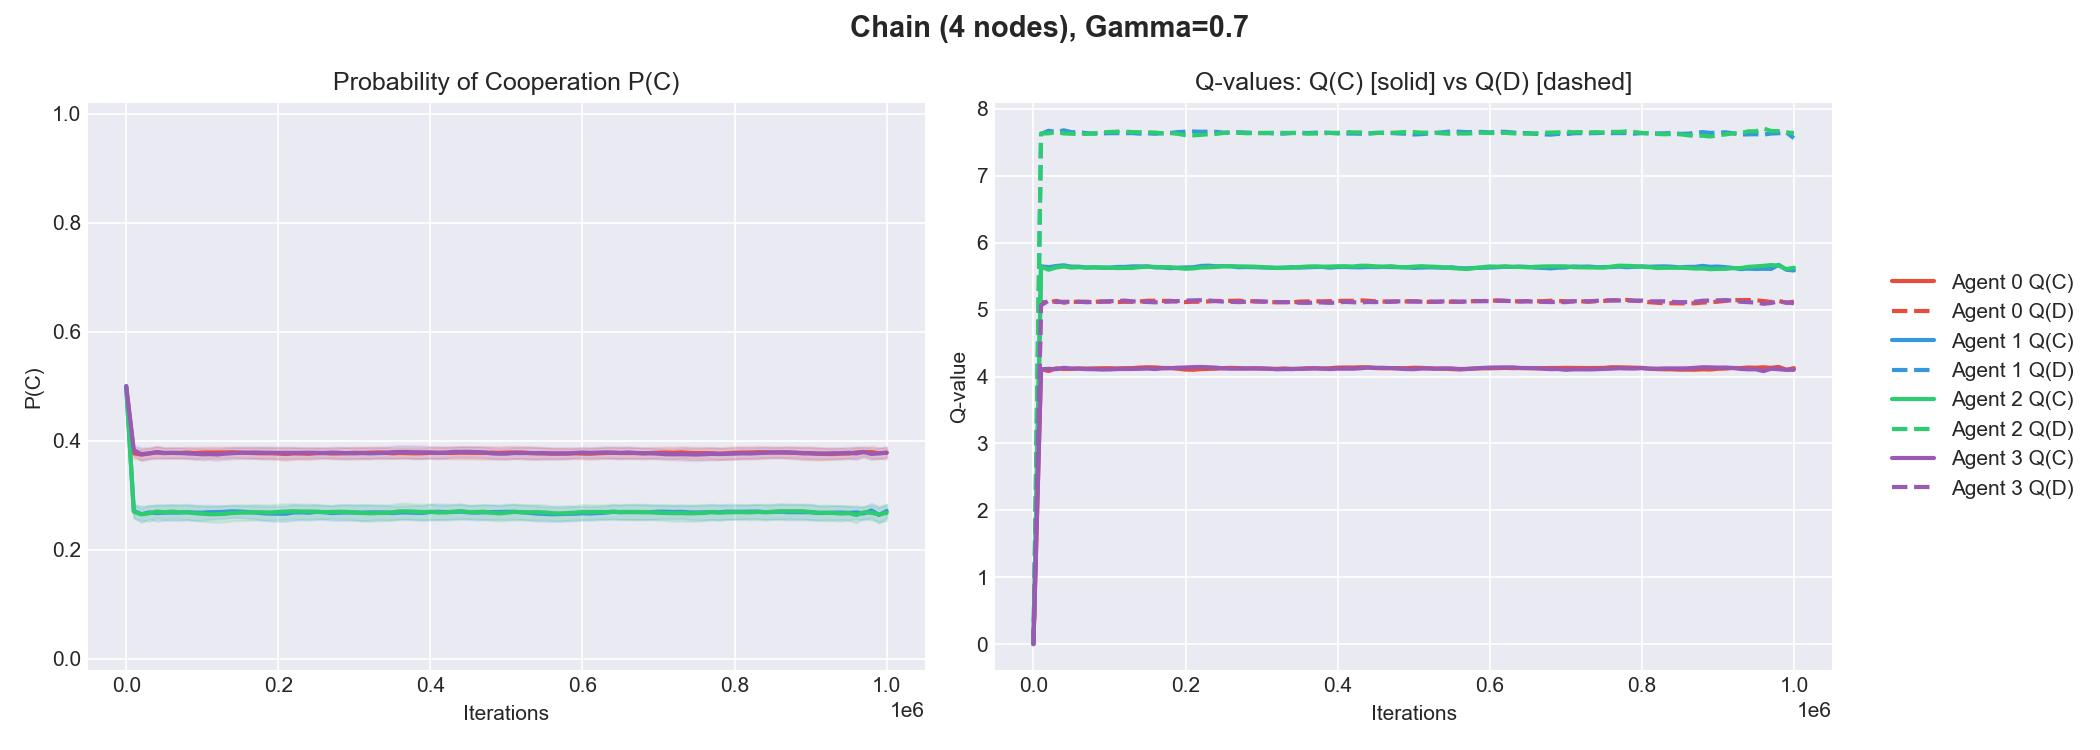
\includegraphics[width=\linewidth]{figures/chain4_gamma0.7.jpg}
	\caption{Динамика вероятности выбора действия C $p_i^{(t)}(C)$ и Q-значений $Q_i^{(t)}(a)$ алгоритма Q-обучения при $\gamma=0.7$. $T=1000000$, $\alpha = 0.01, \beta = 0.5$.}
\end{figure}

\begin{figure} [H]
	\centering
	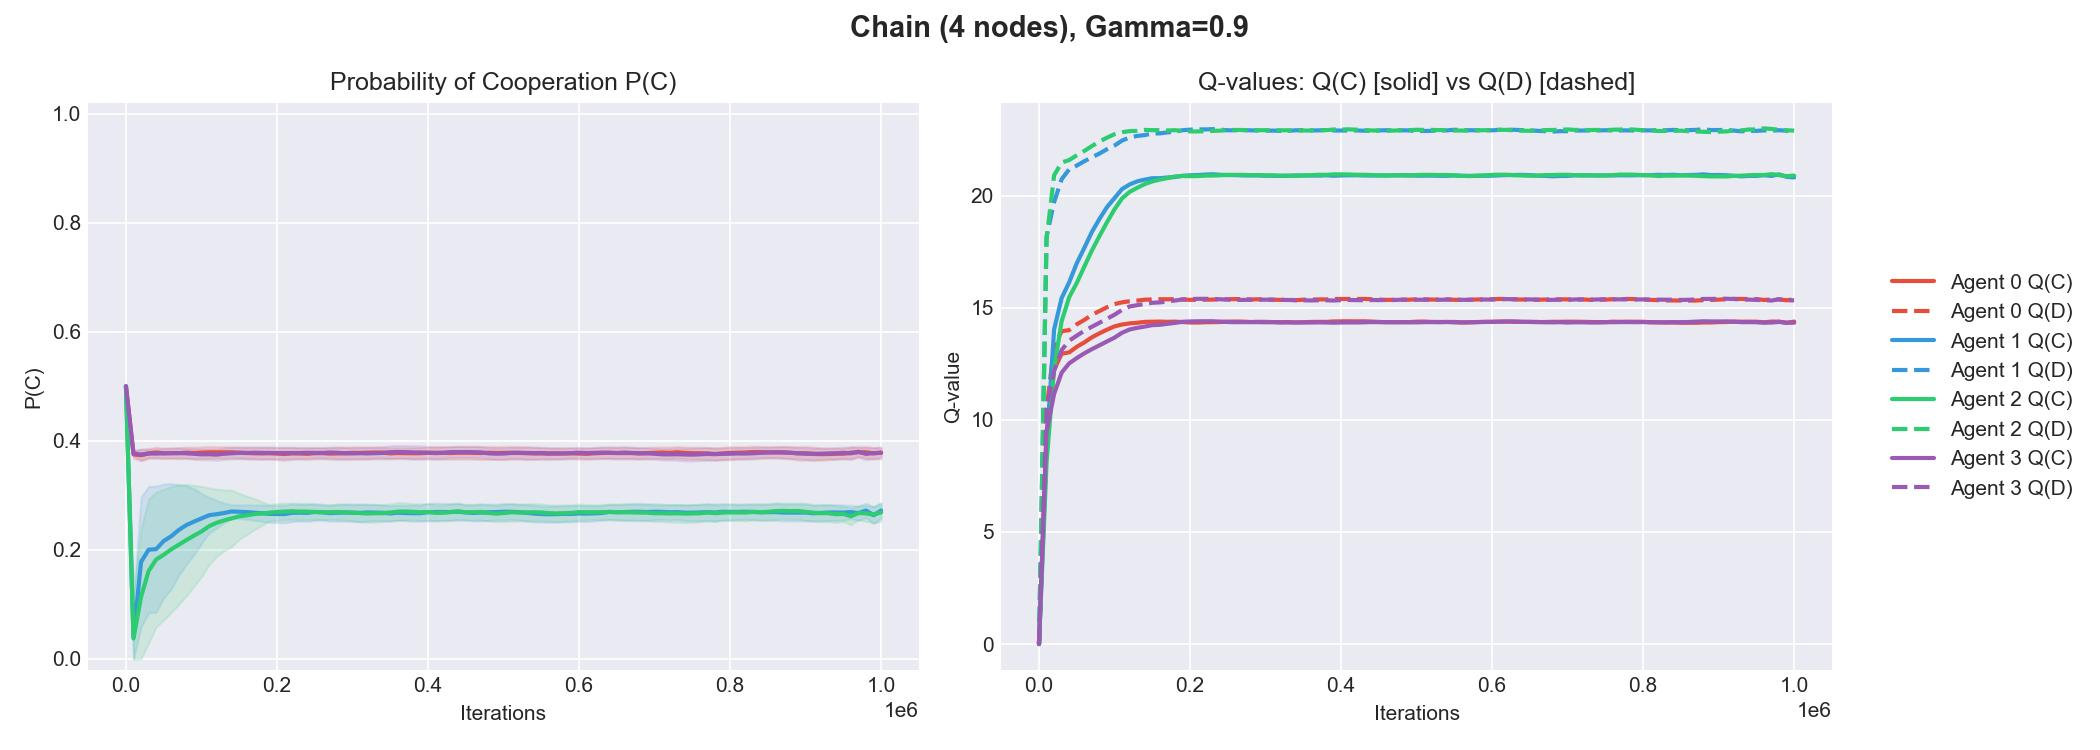
\includegraphics[width=\linewidth]{figures/chain4_gamma0.9.jpg}
	\caption{Динамика вероятности выбора действия C $p_i^{(t)}(C)$ и Q-значений $Q_i^{(t)}(a)$ алгоритма Q-обучения при $\gamma=0.9$. $T=1000000$, $\alpha = 0.01, \beta = 0.5$.}
\end{figure}

\subsubsection{Звезда}

\begin{figure} [H]
	\centering
	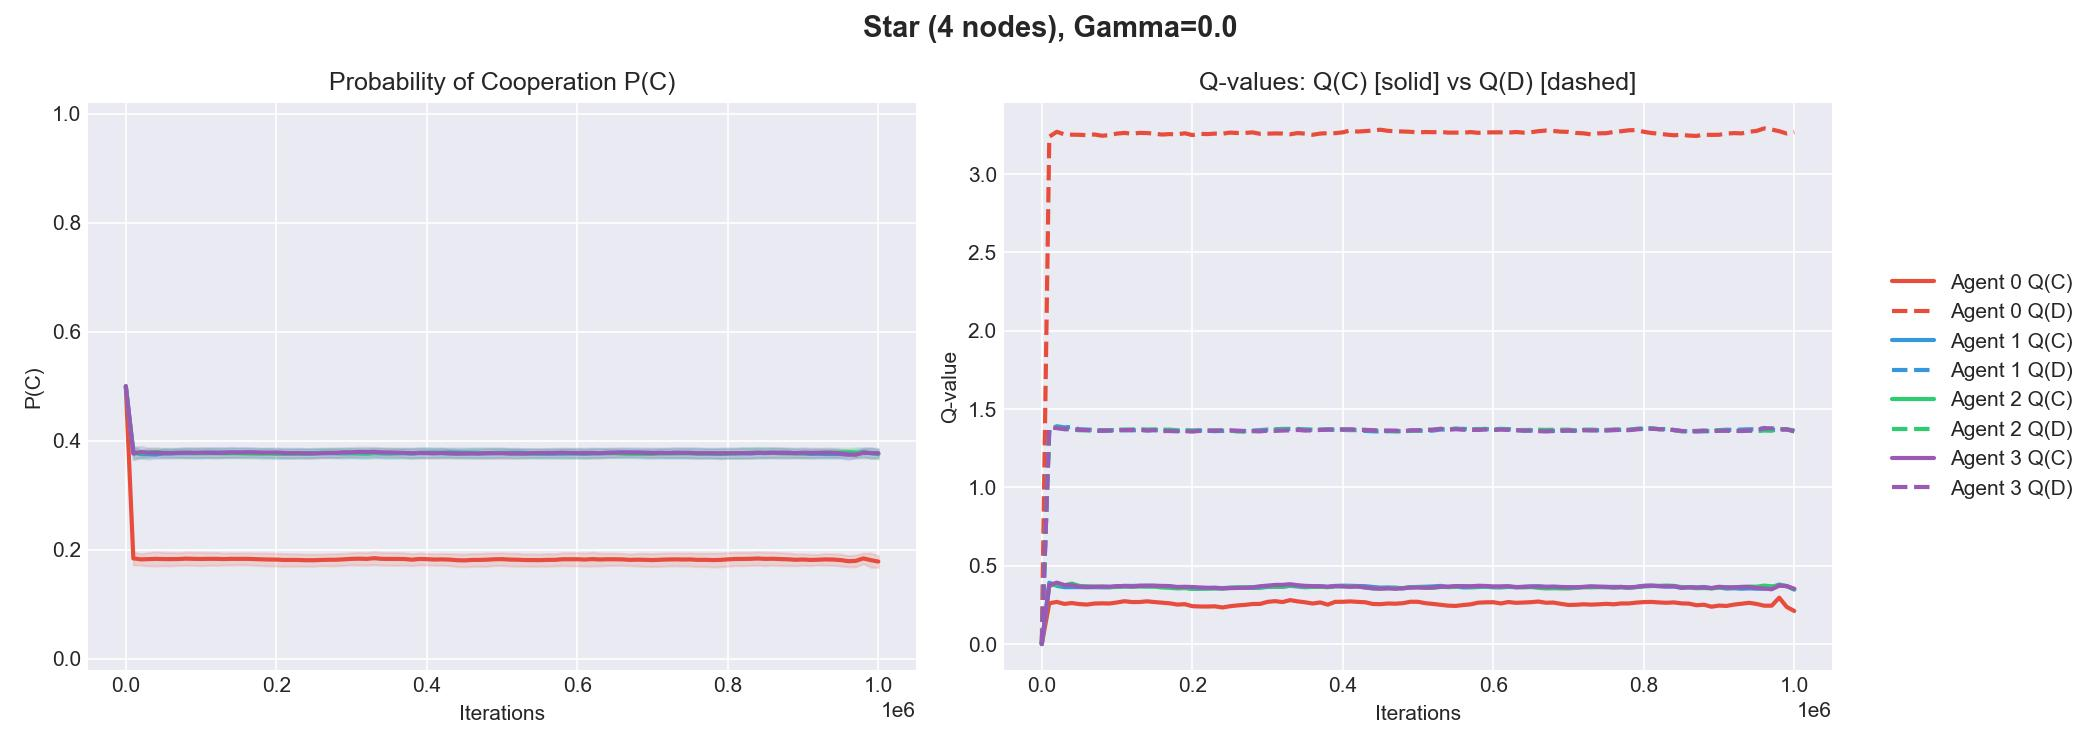
\includegraphics[width=\linewidth]{figures/star4_gamma0.0.jpg}
	\caption{Динамика вероятности выбора действия C $p_i^{(t)}(C)$ и Q-значений $Q_i^{(t)}(a)$ алгоритма Q-обучения при $\gamma=0.0$. $T=1000000$, $\alpha = 0.01, \beta = 0.5$.}
\end{figure}

\begin{figure} [H]
	\centering
	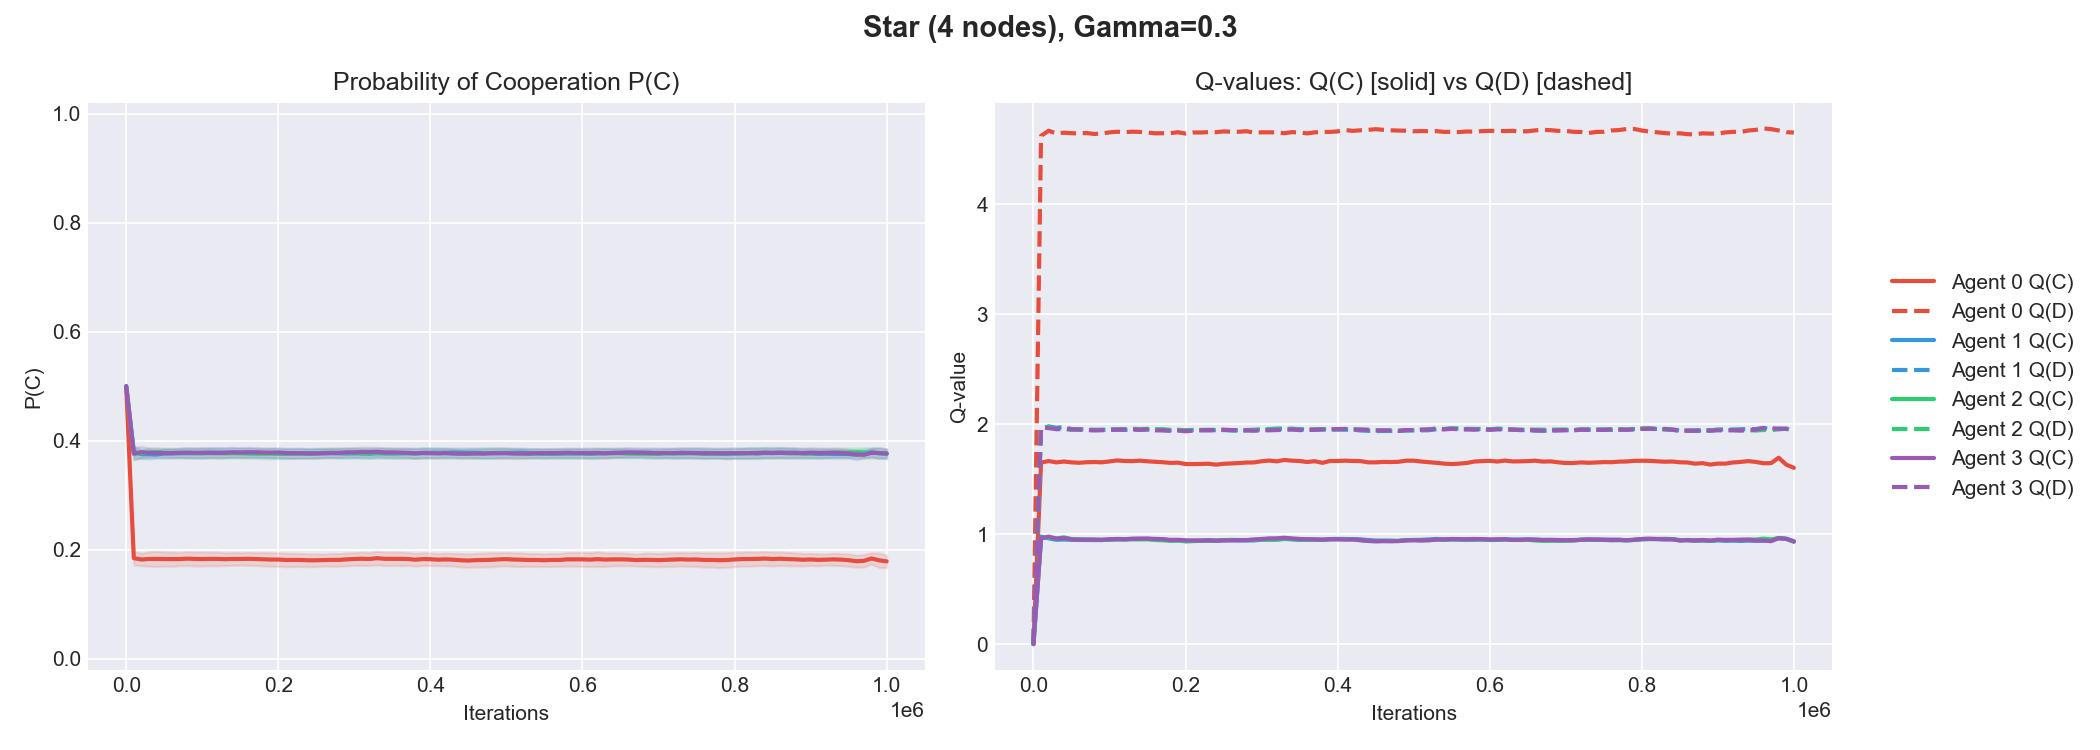
\includegraphics[width=\linewidth]{figures/star4_gamma0.3.jpg}
	\caption{Динамика вероятности выбора действия C $p_i^{(t)}(C)$ и Q-значений $Q_i^{(t)}(a)$ алгоритма Q-обучения при $\gamma=0.3$. $T=1000000$, $\alpha = 0.01, \beta = 0.5$.}
\end{figure}

\begin{figure} [H]
	\centering
	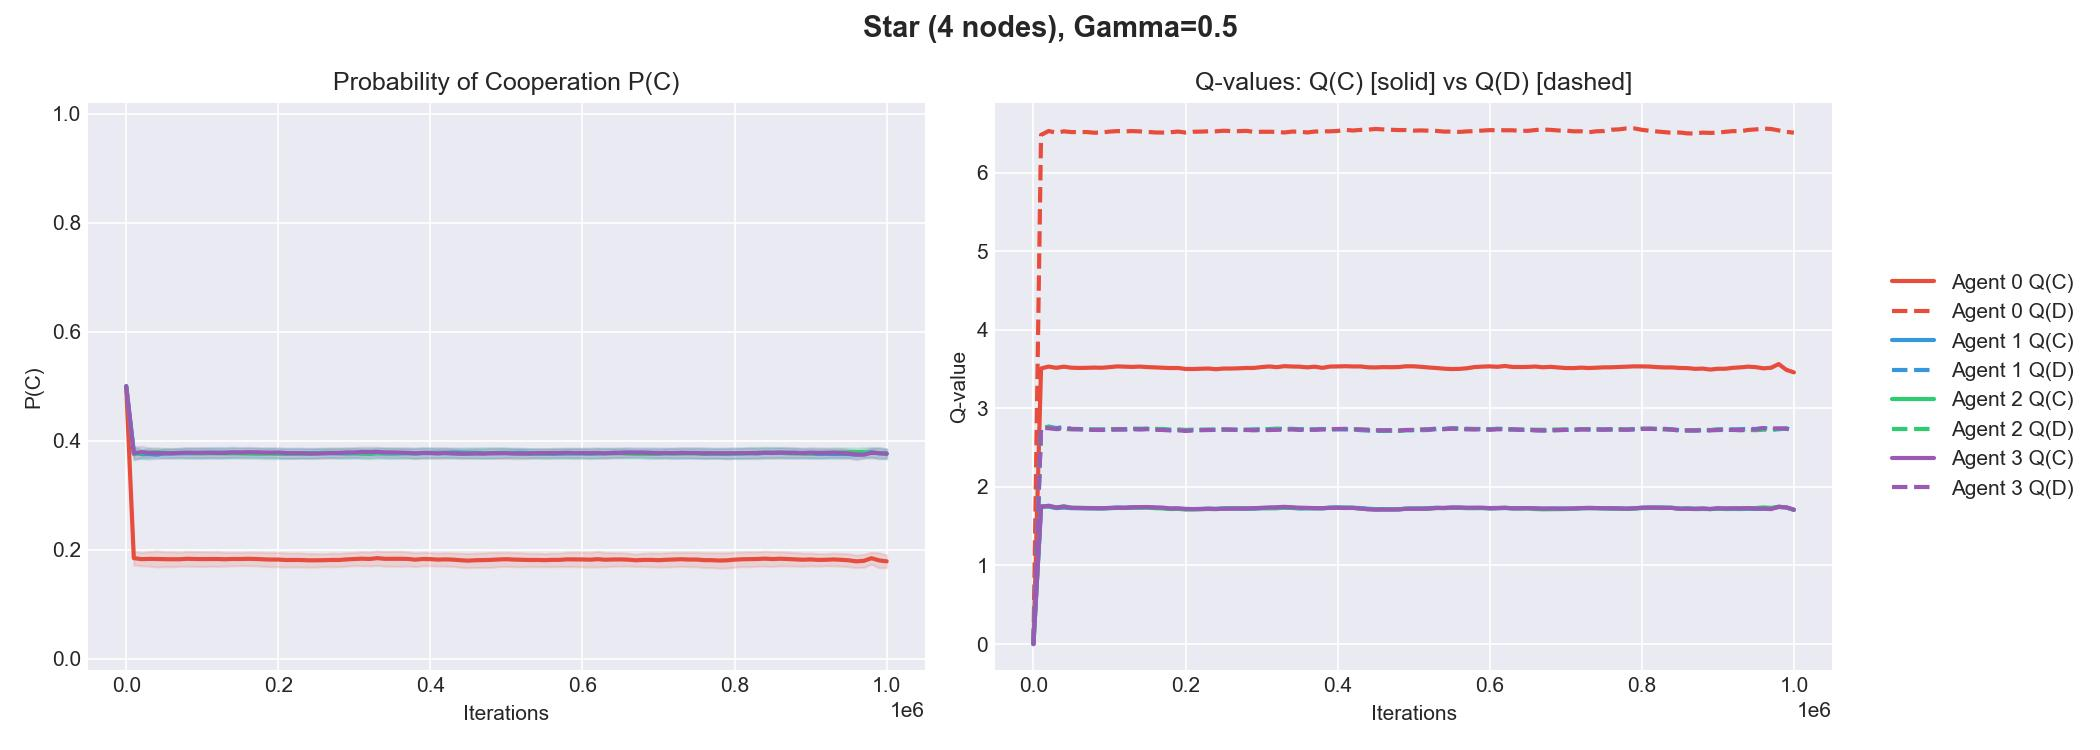
\includegraphics[width=\linewidth]{figures/star4_gamma0.5.jpg}
	\caption{Динамика вероятности выбора действия C $p_i^{(t)}(C)$ и Q-значений $Q_i^{(t)}(a)$ алгоритма Q-обучения при $\gamma=0.5$. $T=1000000$, $\alpha = 0.01, \beta = 0.5$.}
\end{figure}

\begin{figure} [H]
	\centering
	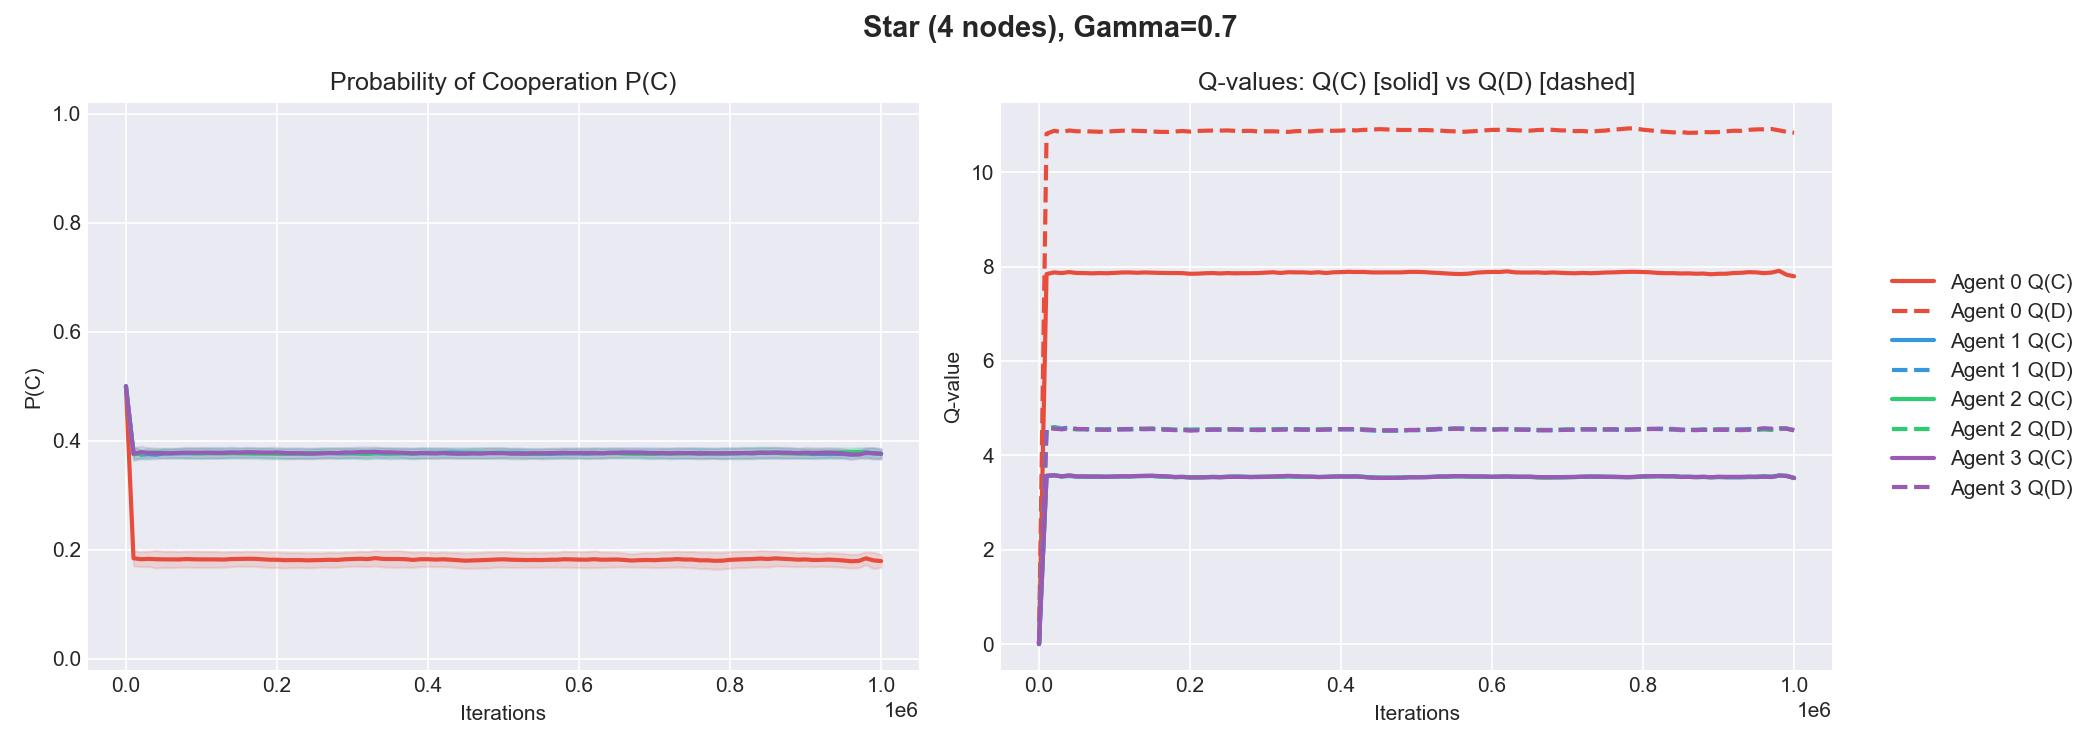
\includegraphics[width=\linewidth]{figures/star4_gamma0.7.jpg}
	\caption{Динамика вероятности выбора действия C $p_i^{(t)}(C)$ и Q-значений $Q_i^{(t)}(a)$ алгоритма Q-обучения при $\gamma=0.7$. $T=1000000$, $\alpha = 0.01, \beta = 0.5$.}
\end{figure}

\begin{figure} [H]
	\centering
	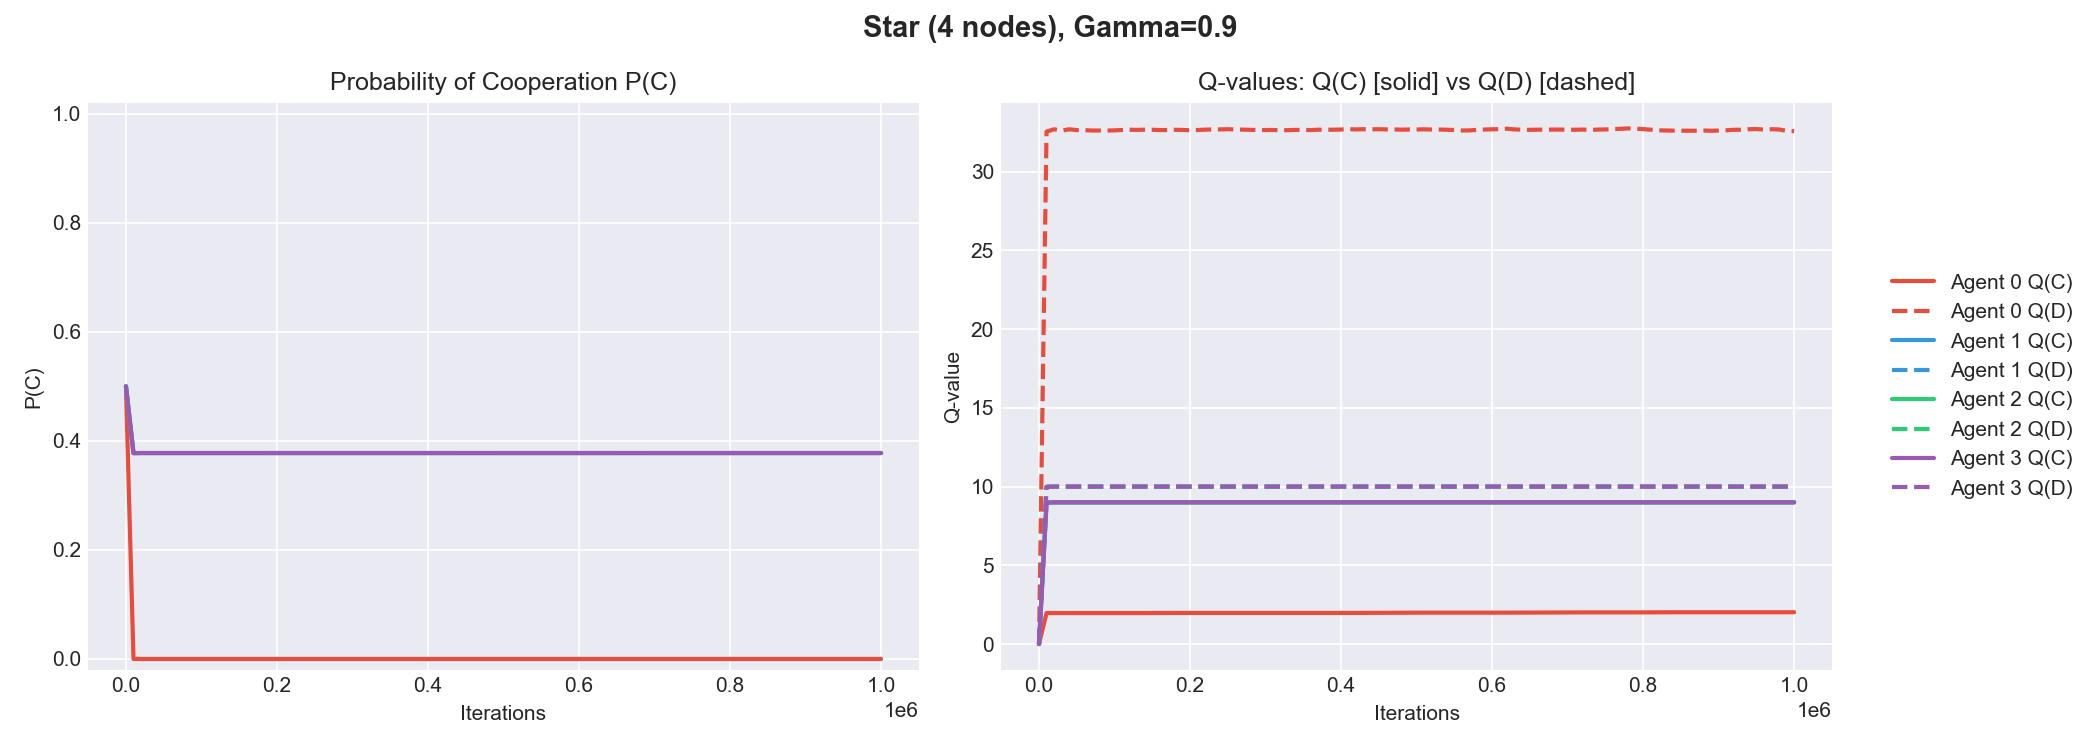
\includegraphics[width=\linewidth]{figures/star4_gamma0.9.jpg}
	\caption{Динамика вероятности выбора действия C $p_i^{(t)}(C)$ и Q-значений $Q_i^{(t)}(a)$ алгоритма Q-обучения при $\gamma=0.9$. $T=1000000$, $\alpha = 0.01, \beta = 0.5$.}
\end{figure}

\subsubsection{Цикл}

\begin{figure} [H]
	\centering
	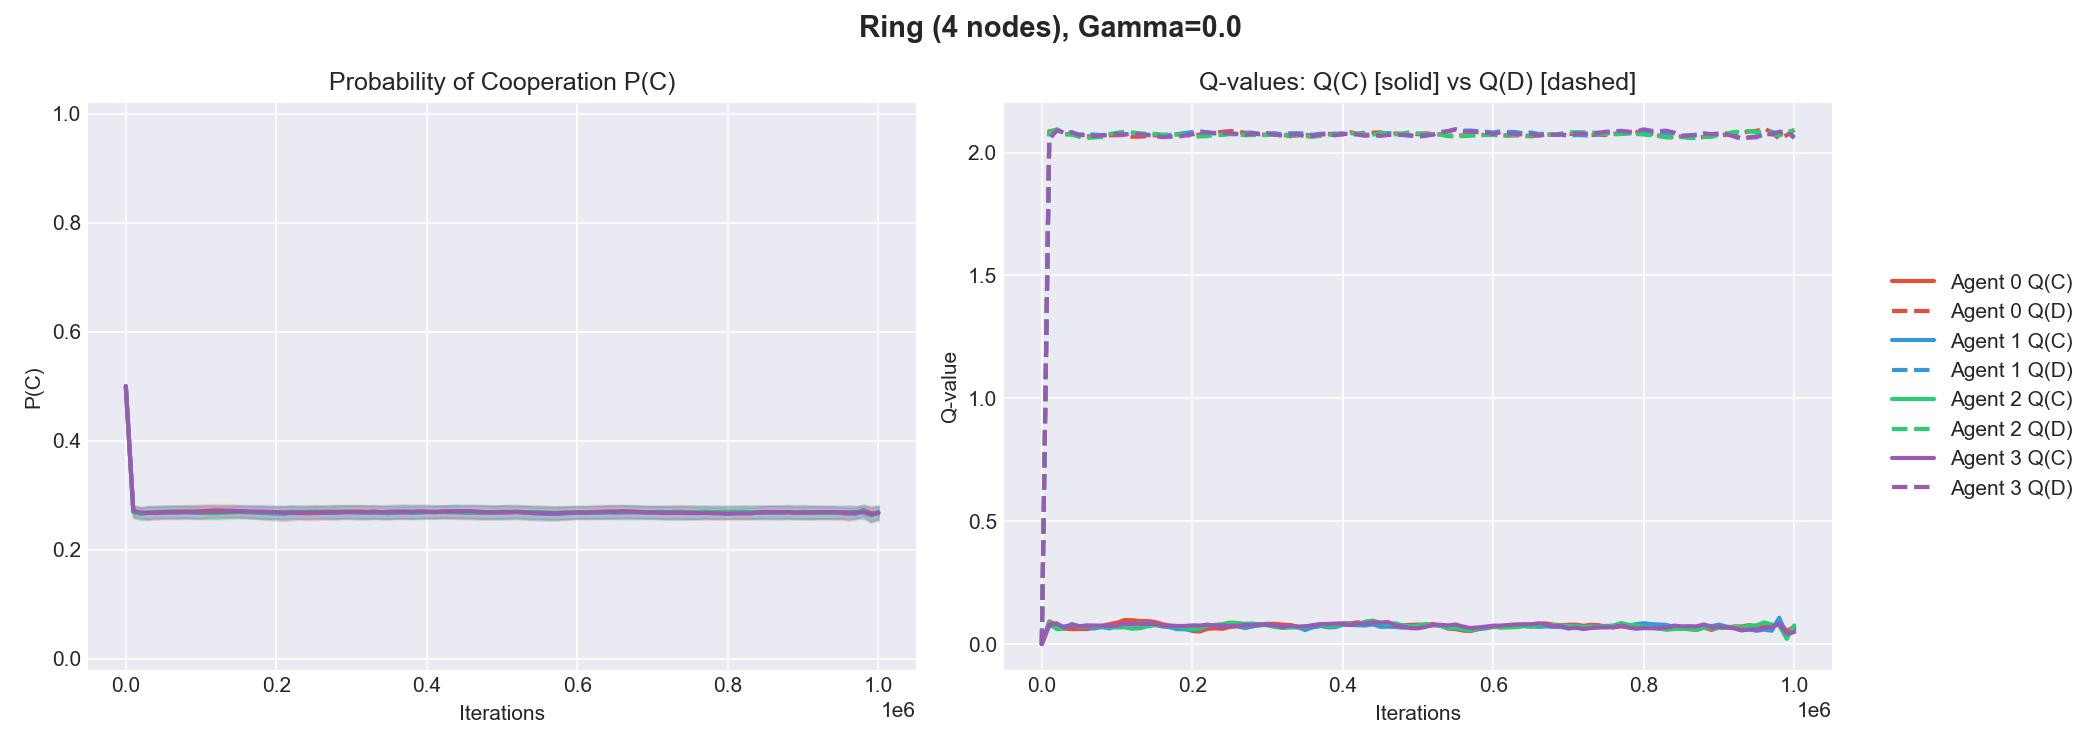
\includegraphics[width=\linewidth]{figures/ring4_gamma0.0.jpg}
	\caption{Динамика вероятности выбора действия C $p_i^{(t)}(C)$ и Q-значений $Q_i^{(t)}(a)$ алгоритма Q-обучения при $\gamma=0.0$. $T=1000000$, $\alpha = 0.01, \beta = 0.5$.}
\end{figure}

\begin{figure} [H]
	\centering
	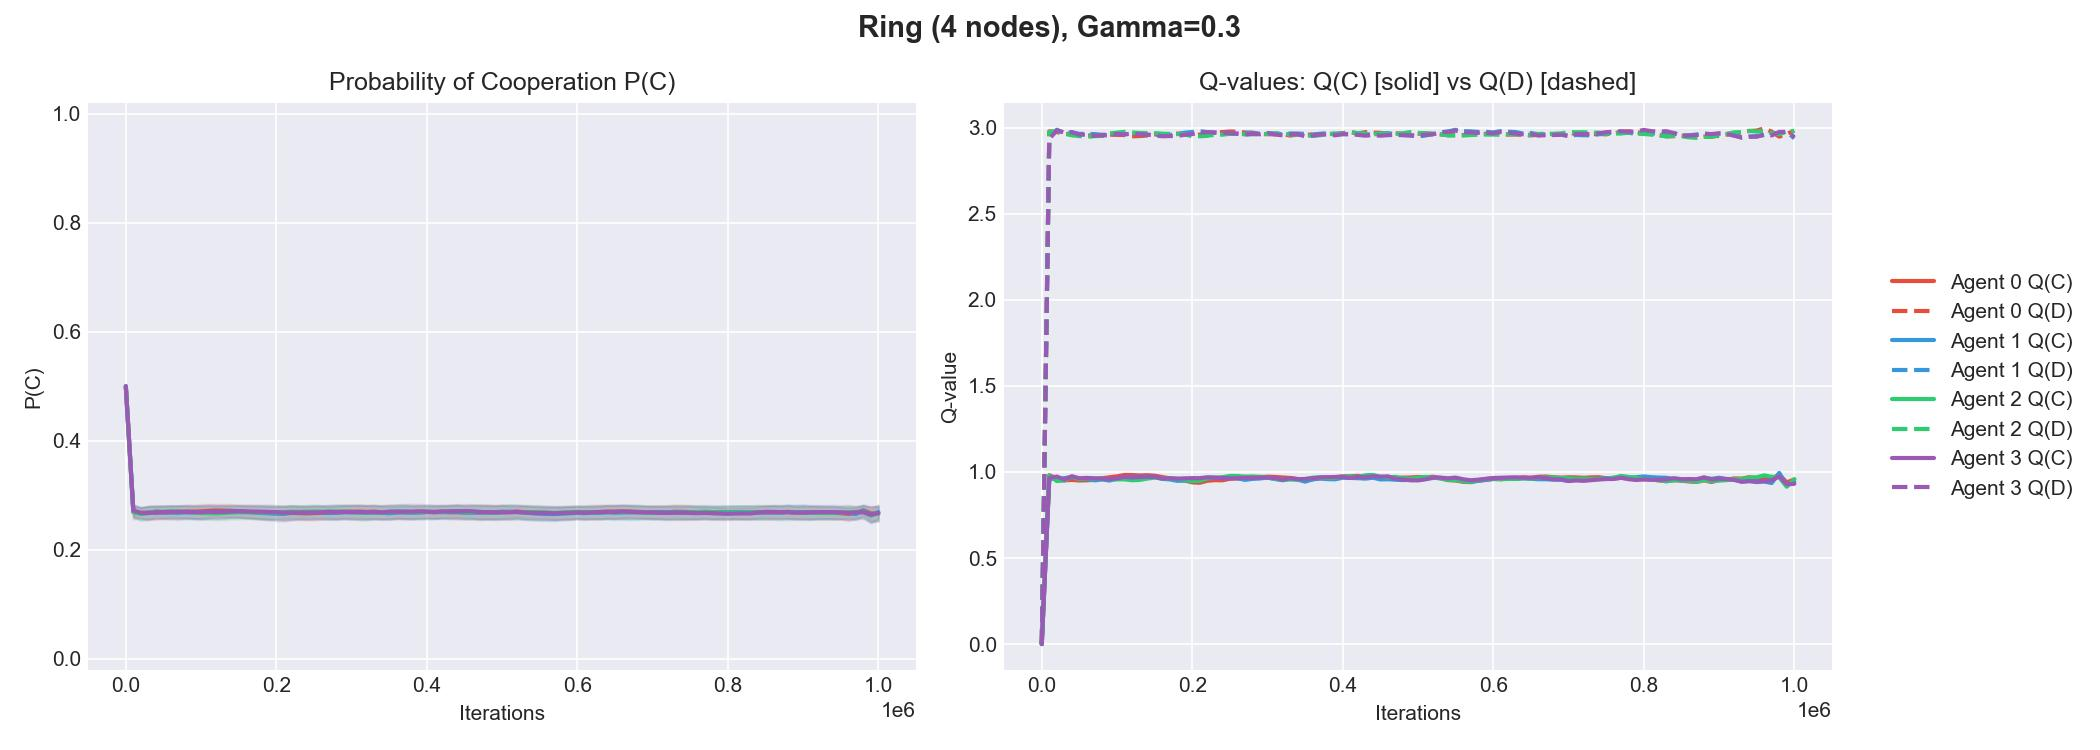
\includegraphics[width=\linewidth]{figures/ring4_gamma0.3.jpg}
	\caption{Динамика вероятности выбора действия C $p_i^{(t)}(C)$ и Q-значений $Q_i^{(t)}(a)$ алгоритма Q-обучения при $\gamma=0.3$. $T=1000000$, $\alpha = 0.01, \beta = 0.5$.}
\end{figure}

\begin{figure} [H]
	\centering
	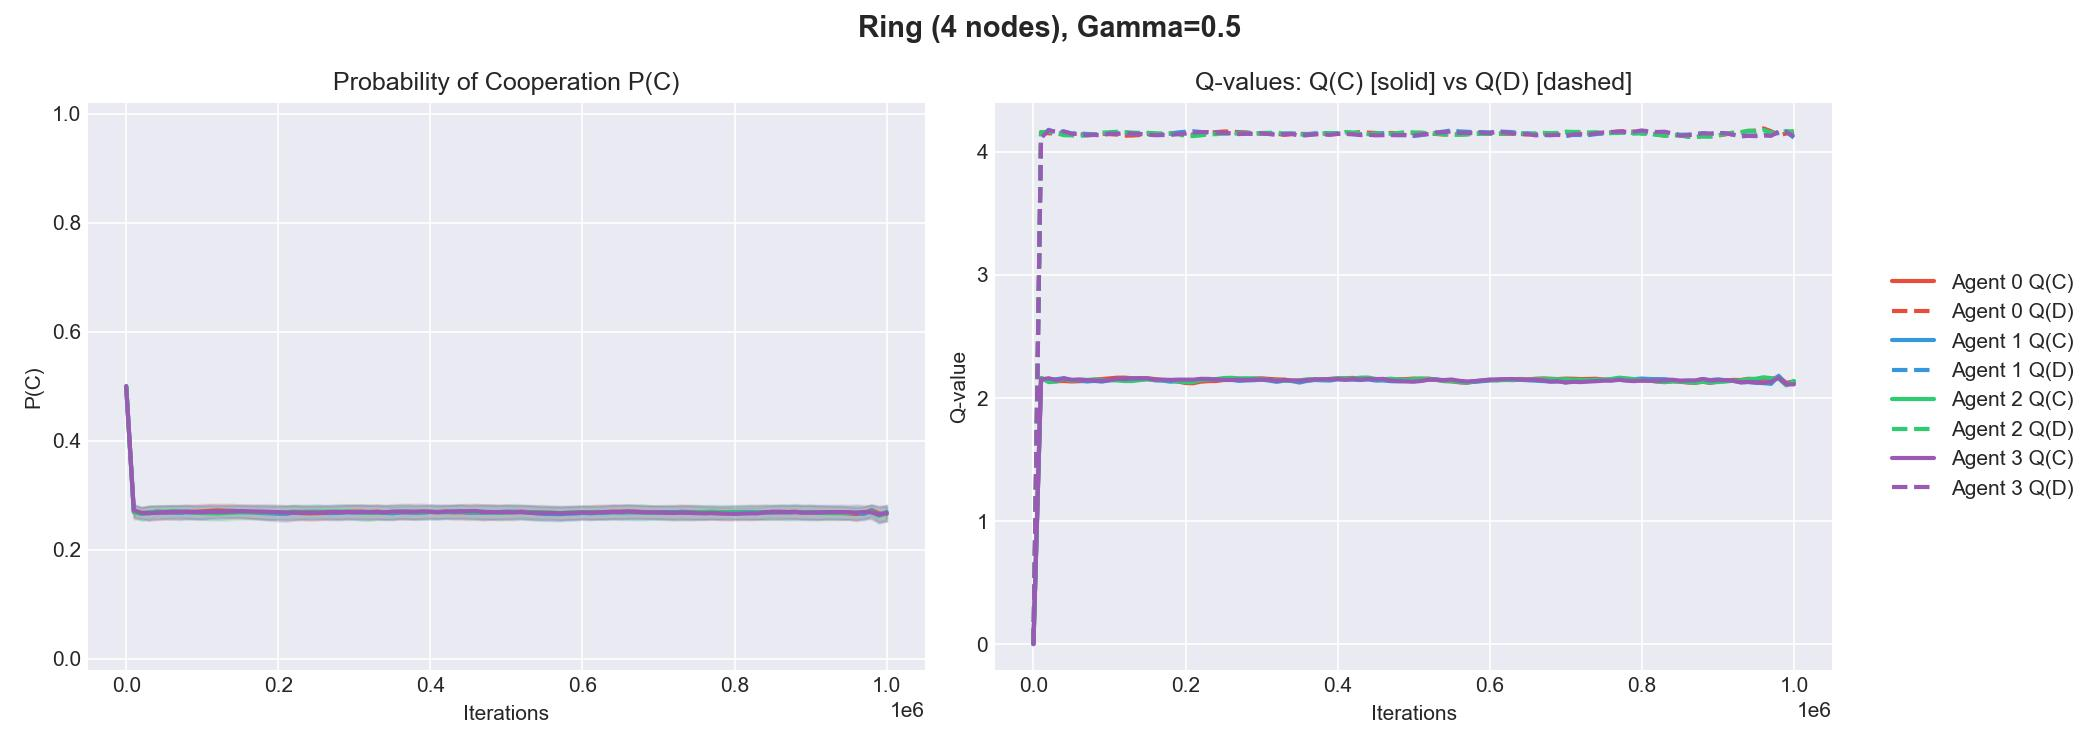
\includegraphics[width=\linewidth]{figures/ring4_gamma0.5.jpg}
	\caption{Динамика вероятности выбора действия C $p_i^{(t)}(C)$ и Q-значений $Q_i^{(t)}(a)$ алгоритма Q-обучения при $\gamma=0.5$. $T=1000000$, $\alpha = 0.01, \beta = 0.5$.}
\end{figure}

\begin{figure} [H]
	\centering
	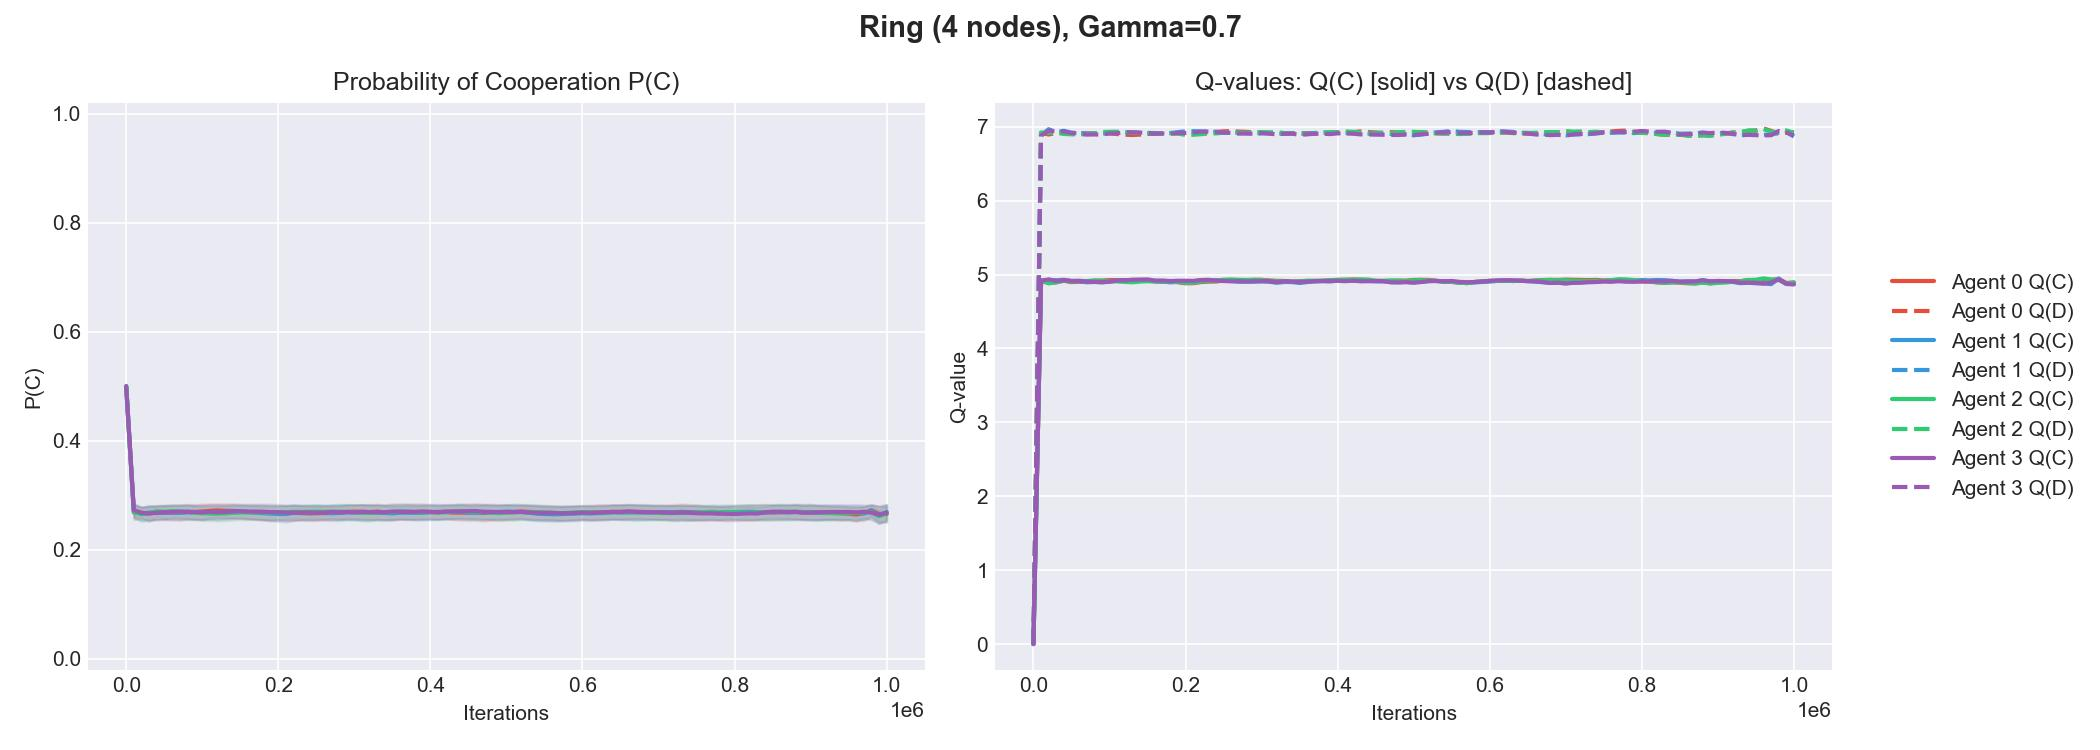
\includegraphics[width=\linewidth]{figures/ring4_gamma0.7.jpg}
	\caption{Динамика вероятности выбора действия C $p_i^{(t)}(C)$ и Q-значений $Q_i^{(t)}(a)$ алгоритма Q-обучения при $\gamma=0.7$. $T=1000000$, $\alpha = 0.01, \beta = 0.5$.}
\end{figure}

\begin{figure} [H]
	\centering
	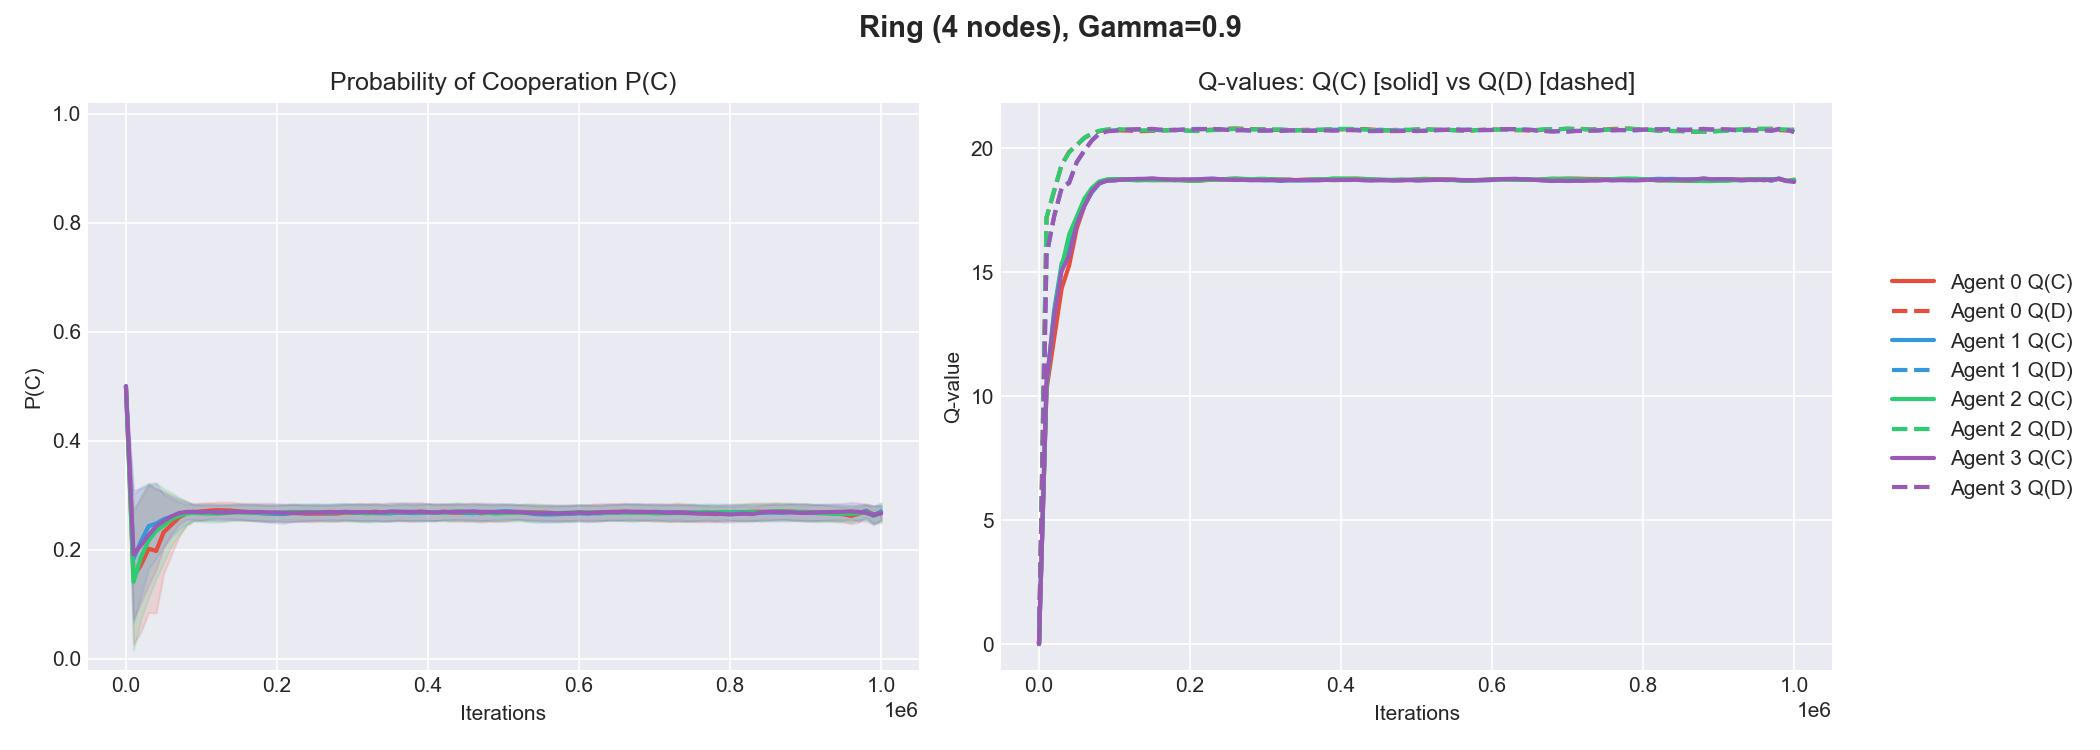
\includegraphics[width=\linewidth]{figures/ring4_gamma0.9.jpg}
	\caption{Динамика вероятности выбора действия C $p_i^{(t)}(C)$ и Q-значений $Q_i^{(t)}(a)$ алгоритма Q-обучения при $\gamma=0.9$. $T=1000000$, $\alpha = 0.01, \beta = 0.5$.}
\end{figure}

\subsubsection{Колесо}

\begin{figure} [H]
	\centering
	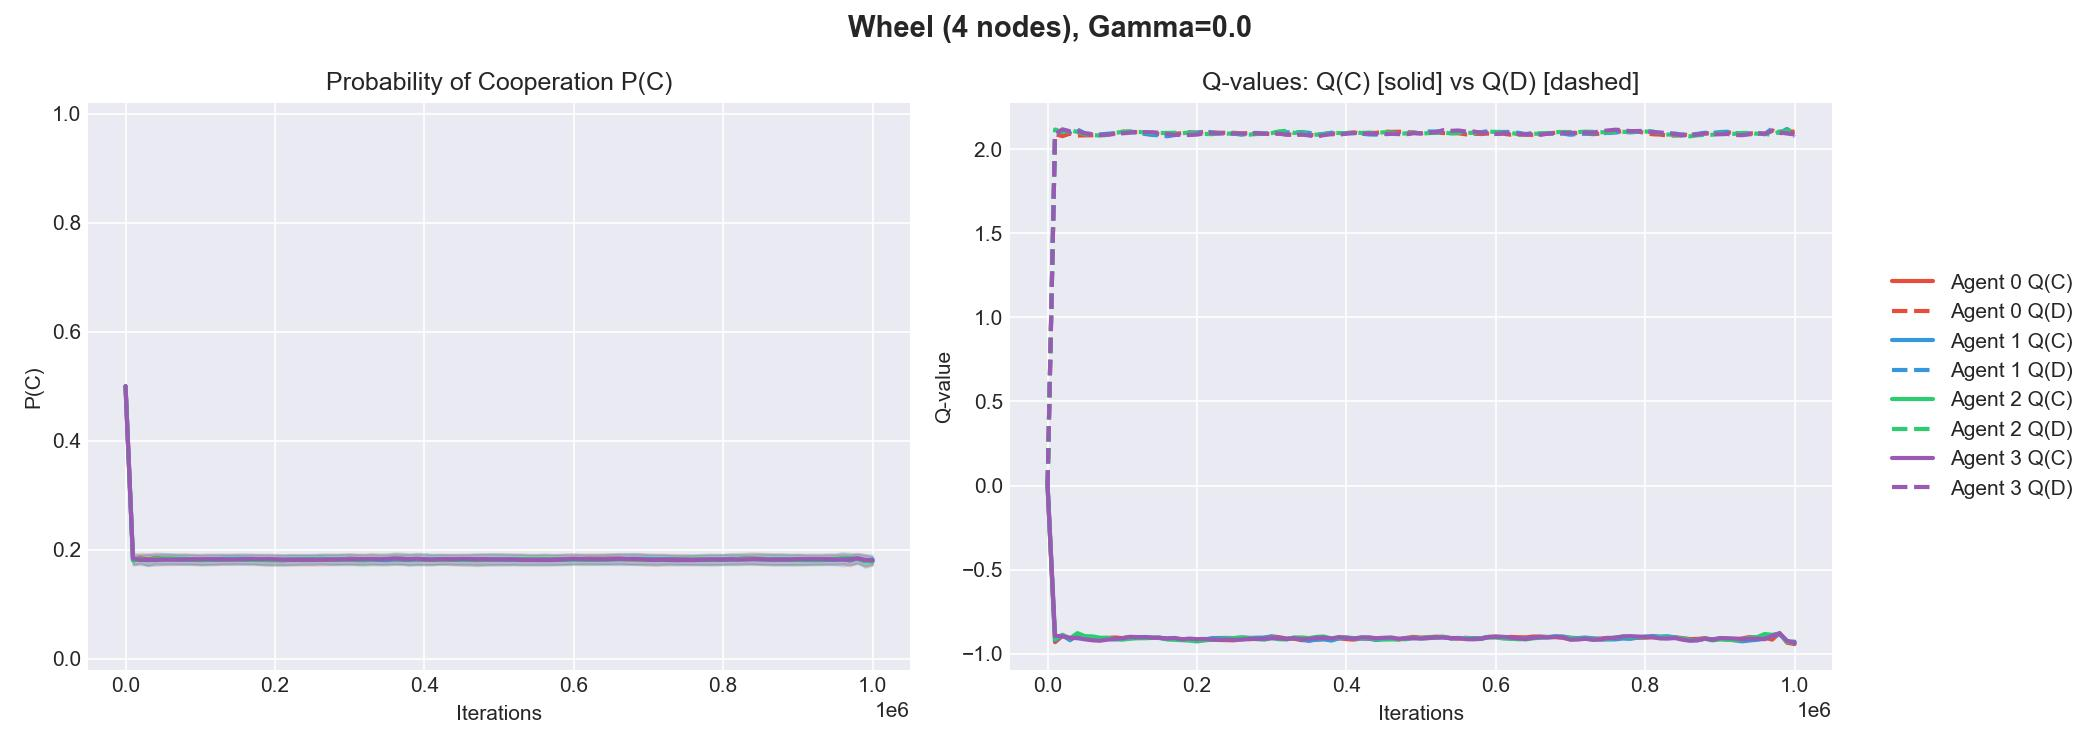
\includegraphics[width=\linewidth]{figures/wheel4_gamma0.0.jpg}
	\caption{Динамика вероятности выбора действия C $p_i^{(t)}(C)$ и Q-значений $Q_i^{(t)}(a)$ алгоритма Q-обучения при $\gamma=0.0$. $T=1000000$, $\alpha = 0.01, \beta = 0.5$.}
\end{figure}

\begin{figure} [H]
	\centering
	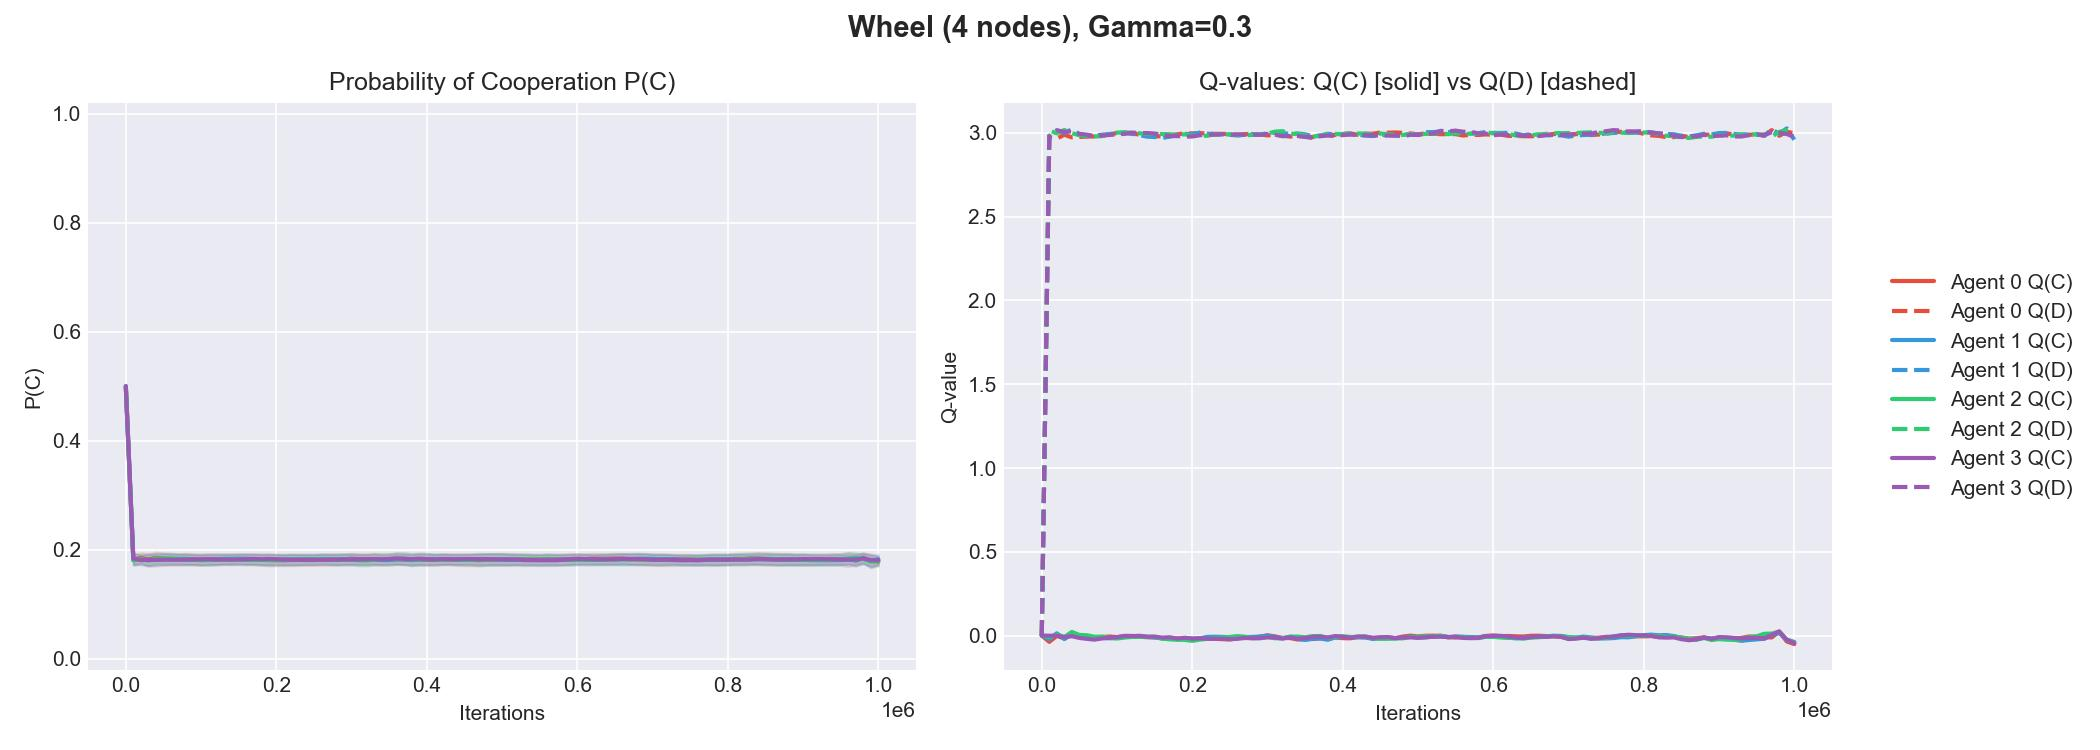
\includegraphics[width=\linewidth]{figures/wheel4_gamma0.3.jpg}
	\caption{Динамика вероятности выбора действия C $p_i^{(t)}(C)$ и Q-значений $Q_i^{(t)}(a)$ алгоритма Q-обучения при $\gamma=0.3$. $T=1000000$, $\alpha = 0.01, \beta = 0.5$.}
\end{figure}

\begin{figure} [H]
	\centering
	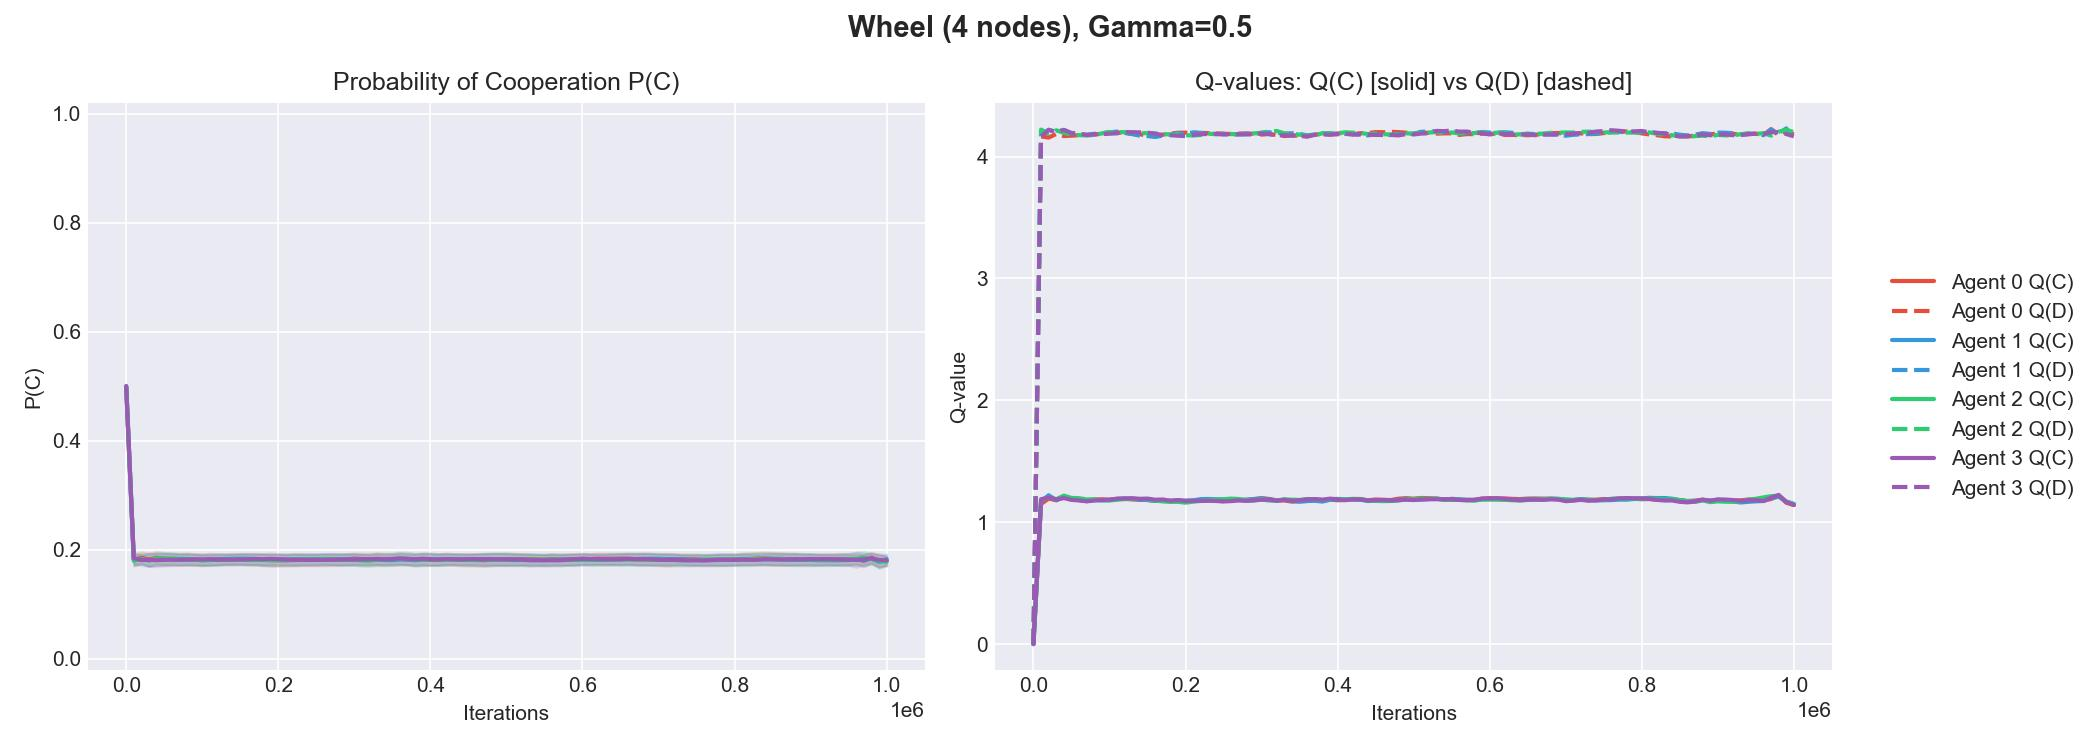
\includegraphics[width=\linewidth]{figures/wheel4_gamma0.5.jpg}
	\caption{Динамика вероятности выбора действия C $p_i^{(t)}(C)$ и Q-значений $Q_i^{(t)}(a)$ алгоритма Q-обучения при $\gamma=0.5$. $T=1000000$, $\alpha = 0.01, \beta = 0.5$.}
\end{figure}

\begin{figure} [H]
	\centering
	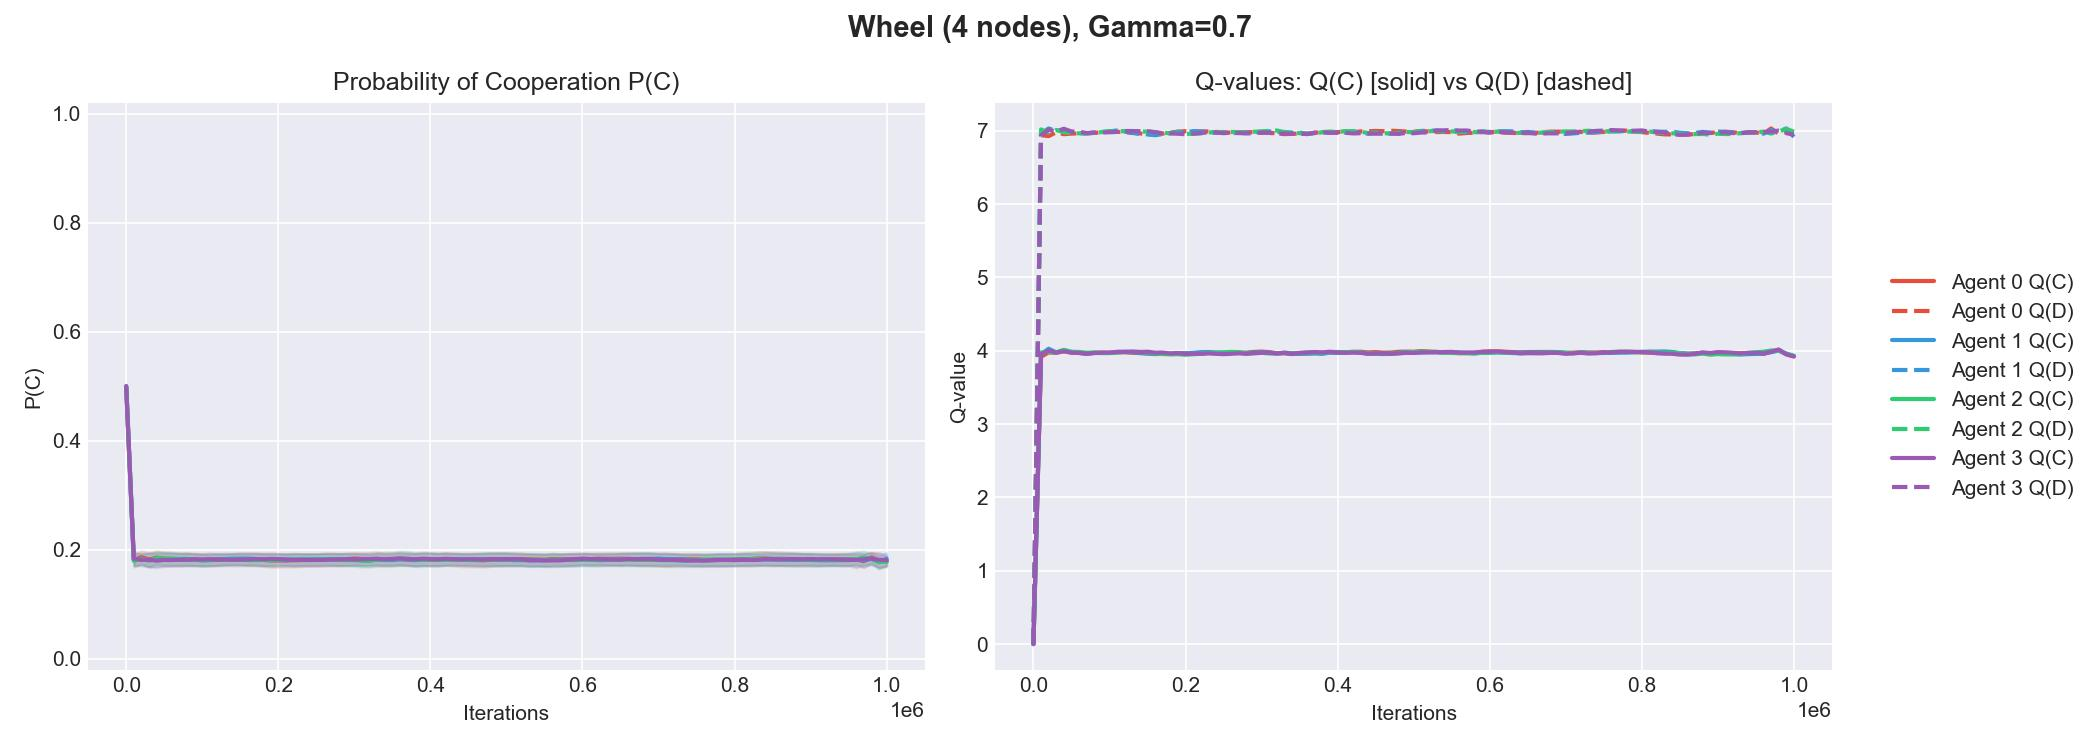
\includegraphics[width=\linewidth]{figures/wheel4_gamma0.7.jpg}
	\caption{Динамика вероятности выбора действия C $p_i^{(t)}(C)$ и Q-значений $Q_i^{(t)}(a)$ алгоритма Q-обучения при $\gamma=0.7$. $T=1000000$, $\alpha = 0.01, \beta = 0.5$.}
\end{figure}

\begin{figure} [H]
	\centering
	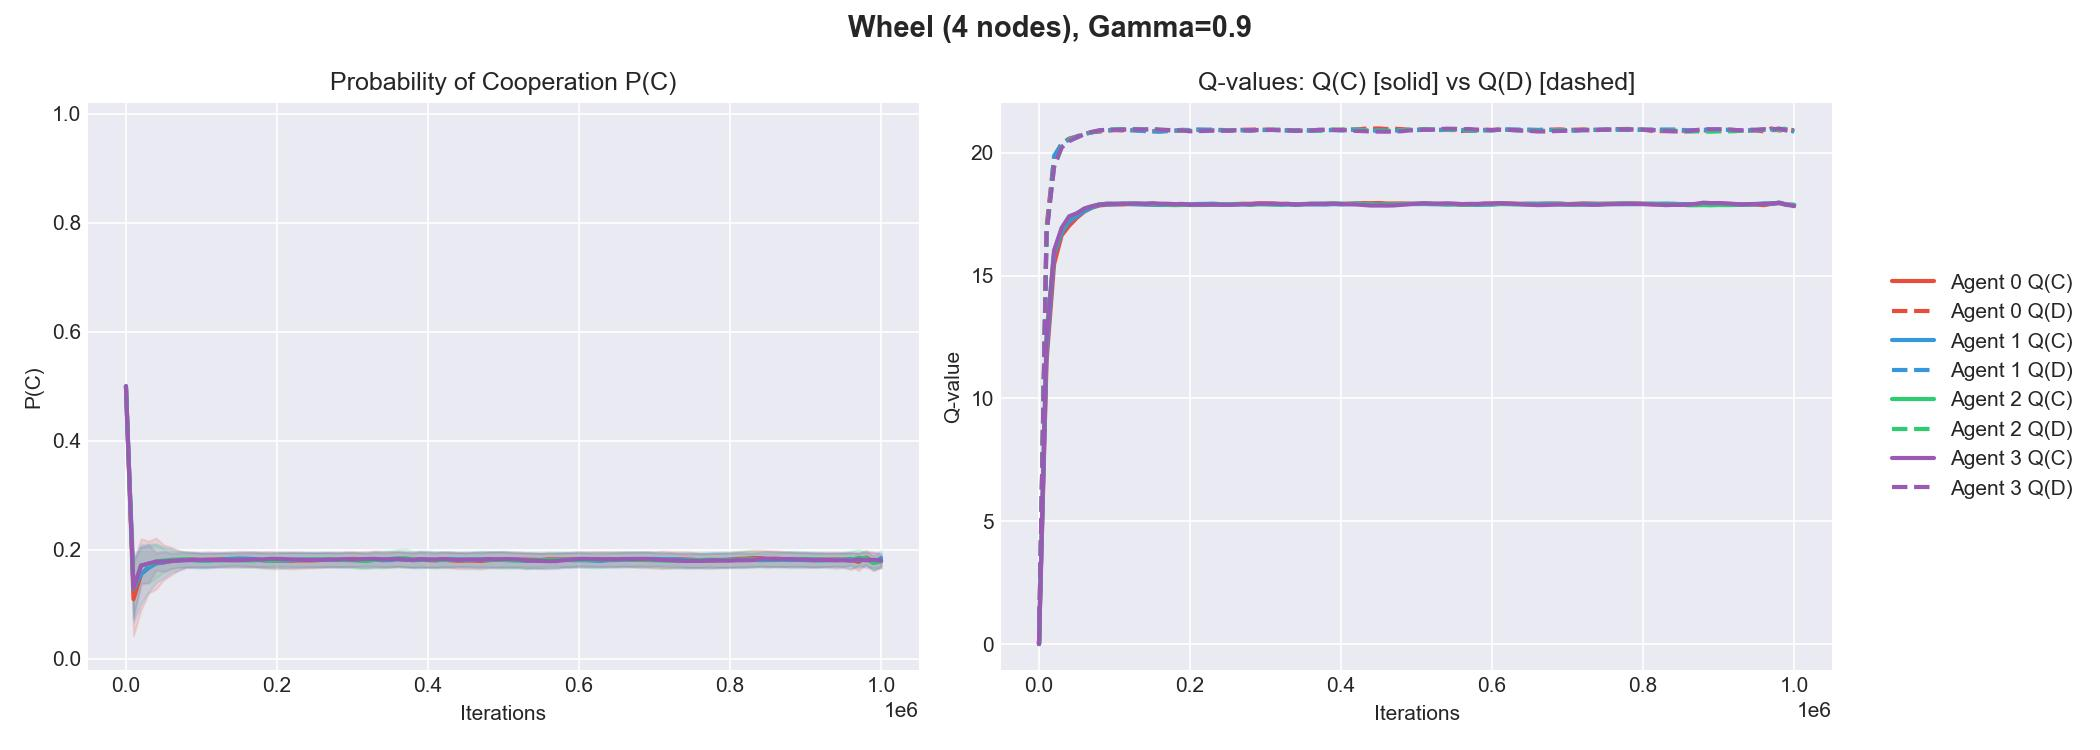
\includegraphics[width=\linewidth]{figures/wheel4_gamma0.9.jpg}
	\caption{Динамика вероятности выбора действия C $p_i^{(t)}(C)$ и Q-значений $Q_i^{(t)}(a)$ алгоритма Q-обучения при $\gamma=0.9$. $T=1000000$, $\alpha = 0.01, \beta = 0.5$.}
\end{figure}


lain}
\bibliography{ref}

\end{document}
